% slides_example.tex
%
% Example .tex file for the beamer-purdue theme
%
% Copyright (c) 2016 Dennis Ogbe <dogbe@purdue.edu>
%
% This file is published under the Creative Commons Attribution-ShareAlike 4.0
% International License. For more information, please visit
% https://creativecommons.org/licenses/by-sa/4.0/
%
% See the README.md for usage instructions. This style really only has one
% option: When called with the "altlogo" option, it will use the "Purdue
% University" logo instead of the "Purdue Engineering" logo.

% we want serif math fonts, they look better
\documentclass[pdf, mathserif]{beamer}

% load required packages. I prefer IEEEtran for equations, but that's a
% personal preference.
\usepackage{IEEEtrantools}

\usepackage{pgf}  % PGF/TikZ is needed for nice plots

\usepackage[cmex10]{mathtools} % for math equations
\usepackage{amssymb}
\usepackage{bm}

% theorems - can use \begin{IEEEproof} as alternative to \begin{proof}
\usepackage{amsthm}
\renewcommand{\qedsymbol}{$\blacksquare$} % want a black square for proofs

% useful to set this when using Inkscape SVG figures
\graphicspath{{./graphics/}}

% tell beamer to use the purdue-gold theme
% \usetheme[altlogo]{purduegold}
\usetheme{purduegold}


% set title and author
\title{beamer-purdue}
\subtitle{A Beamer template inspired by the Purdue Visual Identity}
\author{Dennis Ogbe}

% let's get started
\begin{document}

\begin{frame}[plain]
  \titlepage
\end{frame}

\begin{frame}
  \frametitle{Overview}
  \tableofcontents
\end{frame}

\section{Examples}
\label{sec:examples}

\begin{frame}
  \frametitle{Hello!}
  \framesubtitle{The \texttt{beamer-purdue} template}

  This is the \texttt{beamer-purdue} Theme. A Beamer template inspired
  by the Purdue Visual Identity.

  An itemized list looks as follows:
  \begin{itemize}
  \item Item 1
  \item Item 2
  \end{itemize}

  The continuous-time Fourier Transform of a signal $x(t)$ is defined as

  \begin{IEEEeqnarray}{rCl}
    \label{eq:ft}
    X(\omega) = \int_{-\infty}^{\infty} x(t)e^{-j\omega t}\ \mathrm{dt}
  \end{IEEEeqnarray}

\end{frame}

\begin{frame}
  \frametitle{A Theorem in a Box}

  \begin{theorem}
    The Bessel functions of the first kind $J_{v}(x)$ are defined as the
    solutions to the Bessel differential equation
    \begin{IEEEeqnarray}{rCl}
      \label{eq:bessel}
      x^{2} \frac{d^{2}\,y}{d\,x^{2}} + x \frac{d\,y}{d\,x} + \left( x^{2} - v^{2} \right)y = 0.
    \end{IEEEeqnarray}
  \end{theorem}
  \begin{IEEEproof}
    Omitted.
  \end{IEEEproof}
\end{frame}

\begin{frame}
  \frametitle{Figures}

  We can include graphics just like we are used to, for example this block
  diagram of an noise-canceling system:
  \begin{center}
    \input{./graphics/anc_bd.pdf_tex}
  \end{center}
\end{frame}

\section{Plots}
\label{sec:plots}

\begin{frame}
  \frametitle{Plotting is fun!}

  On the following pages, we include two examples on how to include plots:
  \begin{enumerate}
    \item A PDF plot
    \item A PGF/TikZ plot
  \end{enumerate}

  PDF plots are nice, but nothing beats the native look of PGF/TikZ. The source
  code to generate both plots can be found in \texttt{extra/plot\_bessel.py}
\end{frame}

\begin{frame}
  \frametitle{A PDF Plot}
  \begin{center}
    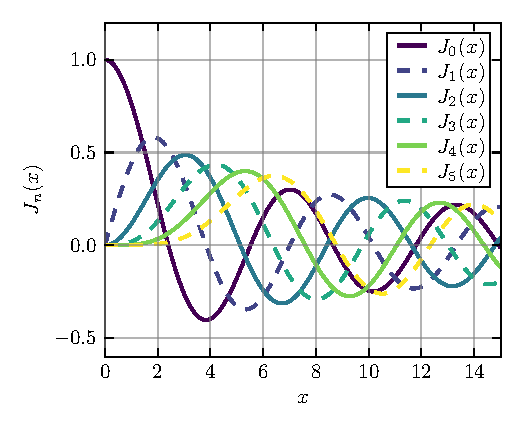
\includegraphics{./plots/bessel.pdf}
  \end{center}
\end{frame}

\begin{frame}
  \frametitle{A PGF/TikZ Plot}
  \begin{center}
    %% Creator: Matplotlib, PGF backend
%%
%% To include the figure in your LaTeX document, write
%%   \input{<filename>.pgf}
%%
%% Make sure the required packages are loaded in your preamble
%%   \usepackage{pgf}
%%
%% Figures using additional raster images can only be included by \input if
%% they are in the same directory as the main LaTeX file. For loading figures
%% from other directories you can use the `import` package
%%   \usepackage{import}
%% and then include the figures with
%%   \import{<path to file>}{<filename>.pgf}
%%
%% Matplotlib used the following preamble
%%   \usepackage[utf8x]{inputenc}
%%   \usepackage[T1]{fontenc}
%%
\begingroup%
\makeatletter%
\begin{pgfpicture}%
\pgfpathrectangle{\pgfpointorigin}{\pgfqpoint{3.486924in}{2.905770in}}%
\pgfusepath{use as bounding box, clip}%
\begin{pgfscope}%
\pgfsetbuttcap%
\pgfsetmiterjoin%
\definecolor{currentfill}{rgb}{1.000000,1.000000,1.000000}%
\pgfsetfillcolor{currentfill}%
\pgfsetlinewidth{0.000000pt}%
\definecolor{currentstroke}{rgb}{1.000000,1.000000,1.000000}%
\pgfsetstrokecolor{currentstroke}%
\pgfsetdash{}{0pt}%
\pgfpathmoveto{\pgfqpoint{0.000000in}{0.000000in}}%
\pgfpathlineto{\pgfqpoint{3.486924in}{0.000000in}}%
\pgfpathlineto{\pgfqpoint{3.486924in}{2.905770in}}%
\pgfpathlineto{\pgfqpoint{0.000000in}{2.905770in}}%
\pgfpathclose%
\pgfusepath{fill}%
\end{pgfscope}%
\begin{pgfscope}%
\pgfsetbuttcap%
\pgfsetmiterjoin%
\definecolor{currentfill}{rgb}{1.000000,1.000000,1.000000}%
\pgfsetfillcolor{currentfill}%
\pgfsetlinewidth{0.000000pt}%
\definecolor{currentstroke}{rgb}{0.000000,0.000000,0.000000}%
\pgfsetstrokecolor{currentstroke}%
\pgfsetstrokeopacity{0.000000}%
\pgfsetdash{}{0pt}%
\pgfpathmoveto{\pgfqpoint{0.699384in}{0.529568in}}%
\pgfpathlineto{\pgfqpoint{3.336924in}{0.529568in}}%
\pgfpathlineto{\pgfqpoint{3.336924in}{2.755770in}}%
\pgfpathlineto{\pgfqpoint{0.699384in}{2.755770in}}%
\pgfpathclose%
\pgfusepath{fill}%
\end{pgfscope}%
\begin{pgfscope}%
\pgfpathrectangle{\pgfqpoint{0.699384in}{0.529568in}}{\pgfqpoint{2.637540in}{2.226203in}} %
\pgfusepath{clip}%
\pgfsetbuttcap%
\pgfsetmiterjoin%
\pgfsetlinewidth{1.505625pt}%
\definecolor{currentstroke}{rgb}{0.267004,0.004874,0.329415}%
\pgfsetstrokecolor{currentstroke}%
\pgfsetdash{}{0pt}%
\pgfpathmoveto{\pgfqpoint{0.699384in}{2.508414in}}%
\pgfpathlineto{\pgfqpoint{0.709935in}{2.507301in}}%
\pgfpathlineto{\pgfqpoint{0.720486in}{2.503965in}}%
\pgfpathlineto{\pgfqpoint{0.731565in}{2.498079in}}%
\pgfpathlineto{\pgfqpoint{0.743171in}{2.489314in}}%
\pgfpathlineto{\pgfqpoint{0.755569in}{2.477046in}}%
\pgfpathlineto{\pgfqpoint{0.768758in}{2.460751in}}%
\pgfpathlineto{\pgfqpoint{0.783002in}{2.439473in}}%
\pgfpathlineto{\pgfqpoint{0.798301in}{2.412482in}}%
\pgfpathlineto{\pgfqpoint{0.814919in}{2.378483in}}%
\pgfpathlineto{\pgfqpoint{0.832857in}{2.336571in}}%
\pgfpathlineto{\pgfqpoint{0.852376in}{2.285183in}}%
\pgfpathlineto{\pgfqpoint{0.874006in}{2.221762in}}%
\pgfpathlineto{\pgfqpoint{0.898010in}{2.144246in}}%
\pgfpathlineto{\pgfqpoint{0.925180in}{2.048757in}}%
\pgfpathlineto{\pgfqpoint{0.957625in}{1.926200in}}%
\pgfpathlineto{\pgfqpoint{1.000885in}{1.753363in}}%
\pgfpathlineto{\pgfqpoint{1.099011in}{1.358616in}}%
\pgfpathlineto{\pgfqpoint{1.132775in}{1.233656in}}%
\pgfpathlineto{\pgfqpoint{1.161263in}{1.136449in}}%
\pgfpathlineto{\pgfqpoint{1.186322in}{1.058546in}}%
\pgfpathlineto{\pgfqpoint{1.209007in}{0.995006in}}%
\pgfpathlineto{\pgfqpoint{1.229846in}{0.943028in}}%
\pgfpathlineto{\pgfqpoint{1.249102in}{0.900790in}}%
\pgfpathlineto{\pgfqpoint{1.267039in}{0.866678in}}%
\pgfpathlineto{\pgfqpoint{1.283657in}{0.839718in}}%
\pgfpathlineto{\pgfqpoint{1.299220in}{0.818601in}}%
\pgfpathlineto{\pgfqpoint{1.313728in}{0.802556in}}%
\pgfpathlineto{\pgfqpoint{1.327445in}{0.790631in}}%
\pgfpathlineto{\pgfqpoint{1.340370in}{0.782279in}}%
\pgfpathlineto{\pgfqpoint{1.352768in}{0.776883in}}%
\pgfpathlineto{\pgfqpoint{1.364638in}{0.774095in}}%
\pgfpathlineto{\pgfqpoint{1.376508in}{0.773602in}}%
\pgfpathlineto{\pgfqpoint{1.388378in}{0.775367in}}%
\pgfpathlineto{\pgfqpoint{1.400512in}{0.779457in}}%
\pgfpathlineto{\pgfqpoint{1.413173in}{0.786124in}}%
\pgfpathlineto{\pgfqpoint{1.426626in}{0.795812in}}%
\pgfpathlineto{\pgfqpoint{1.440870in}{0.808879in}}%
\pgfpathlineto{\pgfqpoint{1.456170in}{0.825983in}}%
\pgfpathlineto{\pgfqpoint{1.473052in}{0.848324in}}%
\pgfpathlineto{\pgfqpoint{1.491516in}{0.876613in}}%
\pgfpathlineto{\pgfqpoint{1.511827in}{0.911932in}}%
\pgfpathlineto{\pgfqpoint{1.534776in}{0.956456in}}%
\pgfpathlineto{\pgfqpoint{1.561418in}{1.013205in}}%
\pgfpathlineto{\pgfqpoint{1.594391in}{1.088964in}}%
\pgfpathlineto{\pgfqpoint{1.650576in}{1.224741in}}%
\pgfpathlineto{\pgfqpoint{1.701222in}{1.344768in}}%
\pgfpathlineto{\pgfqpoint{1.733403in}{1.415438in}}%
\pgfpathlineto{\pgfqpoint{1.760308in}{1.469310in}}%
\pgfpathlineto{\pgfqpoint{1.783785in}{1.511521in}}%
\pgfpathlineto{\pgfqpoint{1.805151in}{1.545494in}}%
\pgfpathlineto{\pgfqpoint{1.824671in}{1.572476in}}%
\pgfpathlineto{\pgfqpoint{1.842608in}{1.593628in}}%
\pgfpathlineto{\pgfqpoint{1.859490in}{1.610203in}}%
\pgfpathlineto{\pgfqpoint{1.875317in}{1.622715in}}%
\pgfpathlineto{\pgfqpoint{1.890352in}{1.631831in}}%
\pgfpathlineto{\pgfqpoint{1.904596in}{1.637950in}}%
\pgfpathlineto{\pgfqpoint{1.918577in}{1.641563in}}%
\pgfpathlineto{\pgfqpoint{1.932293in}{1.642809in}}%
\pgfpathlineto{\pgfqpoint{1.946010in}{1.641796in}}%
\pgfpathlineto{\pgfqpoint{1.959726in}{1.638556in}}%
\pgfpathlineto{\pgfqpoint{1.973971in}{1.632879in}}%
\pgfpathlineto{\pgfqpoint{1.988742in}{1.624570in}}%
\pgfpathlineto{\pgfqpoint{2.004305in}{1.613244in}}%
\pgfpathlineto{\pgfqpoint{2.020924in}{1.598366in}}%
\pgfpathlineto{\pgfqpoint{2.038861in}{1.579269in}}%
\pgfpathlineto{\pgfqpoint{2.058380in}{1.555174in}}%
\pgfpathlineto{\pgfqpoint{2.080010in}{1.524843in}}%
\pgfpathlineto{\pgfqpoint{2.104542in}{1.486447in}}%
\pgfpathlineto{\pgfqpoint{2.133030in}{1.437557in}}%
\pgfpathlineto{\pgfqpoint{2.169696in}{1.369912in}}%
\pgfpathlineto{\pgfqpoint{2.281275in}{1.161006in}}%
\pgfpathlineto{\pgfqpoint{2.310554in}{1.112613in}}%
\pgfpathlineto{\pgfqpoint{2.335877in}{1.074938in}}%
\pgfpathlineto{\pgfqpoint{2.358562in}{1.045091in}}%
\pgfpathlineto{\pgfqpoint{2.379137in}{1.021596in}}%
\pgfpathlineto{\pgfqpoint{2.398130in}{1.003173in}}%
\pgfpathlineto{\pgfqpoint{2.416067in}{0.988816in}}%
\pgfpathlineto{\pgfqpoint{2.432949in}{0.978111in}}%
\pgfpathlineto{\pgfqpoint{2.449039in}{0.970507in}}%
\pgfpathlineto{\pgfqpoint{2.464602in}{0.965605in}}%
\pgfpathlineto{\pgfqpoint{2.479638in}{0.963176in}}%
\pgfpathlineto{\pgfqpoint{2.494673in}{0.963011in}}%
\pgfpathlineto{\pgfqpoint{2.509709in}{0.965094in}}%
\pgfpathlineto{\pgfqpoint{2.525008in}{0.969485in}}%
\pgfpathlineto{\pgfqpoint{2.540835in}{0.976383in}}%
\pgfpathlineto{\pgfqpoint{2.557453in}{0.986124in}}%
\pgfpathlineto{\pgfqpoint{2.574862in}{0.998953in}}%
\pgfpathlineto{\pgfqpoint{2.593591in}{1.015586in}}%
\pgfpathlineto{\pgfqpoint{2.613902in}{1.036697in}}%
\pgfpathlineto{\pgfqpoint{2.636059in}{1.063013in}}%
\pgfpathlineto{\pgfqpoint{2.661119in}{1.096352in}}%
\pgfpathlineto{\pgfqpoint{2.690398in}{1.139191in}}%
\pgfpathlineto{\pgfqpoint{2.727855in}{1.198210in}}%
\pgfpathlineto{\pgfqpoint{2.837851in}{1.374049in}}%
\pgfpathlineto{\pgfqpoint{2.867659in}{1.416094in}}%
\pgfpathlineto{\pgfqpoint{2.893245in}{1.448486in}}%
\pgfpathlineto{\pgfqpoint{2.916194in}{1.474074in}}%
\pgfpathlineto{\pgfqpoint{2.937297in}{1.494356in}}%
\pgfpathlineto{\pgfqpoint{2.956816in}{1.510113in}}%
\pgfpathlineto{\pgfqpoint{2.975281in}{1.522205in}}%
\pgfpathlineto{\pgfqpoint{2.992691in}{1.531000in}}%
\pgfpathlineto{\pgfqpoint{3.009309in}{1.536973in}}%
\pgfpathlineto{\pgfqpoint{3.025663in}{1.540506in}}%
\pgfpathlineto{\pgfqpoint{3.041754in}{1.541697in}}%
\pgfpathlineto{\pgfqpoint{3.057844in}{1.540627in}}%
\pgfpathlineto{\pgfqpoint{3.073935in}{1.537322in}}%
\pgfpathlineto{\pgfqpoint{3.090553in}{1.531606in}}%
\pgfpathlineto{\pgfqpoint{3.107699in}{1.523328in}}%
\pgfpathlineto{\pgfqpoint{3.125900in}{1.512000in}}%
\pgfpathlineto{\pgfqpoint{3.145156in}{1.497320in}}%
\pgfpathlineto{\pgfqpoint{3.165731in}{1.478791in}}%
\pgfpathlineto{\pgfqpoint{3.188416in}{1.455281in}}%
\pgfpathlineto{\pgfqpoint{3.213739in}{1.425722in}}%
\pgfpathlineto{\pgfqpoint{3.243018in}{1.388000in}}%
\pgfpathlineto{\pgfqpoint{3.280475in}{1.335861in}}%
\pgfpathlineto{\pgfqpoint{3.336924in}{1.254042in}}%
\pgfpathlineto{\pgfqpoint{3.336924in}{1.254042in}}%
\pgfusepath{stroke}%
\end{pgfscope}%
\begin{pgfscope}%
\pgfpathrectangle{\pgfqpoint{0.699384in}{0.529568in}}{\pgfqpoint{2.637540in}{2.226203in}} %
\pgfusepath{clip}%
\pgfsetbuttcap%
\pgfsetmiterjoin%
\pgfsetlinewidth{1.505625pt}%
\definecolor{currentstroke}{rgb}{0.253935,0.265254,0.529983}%
\pgfsetstrokecolor{currentstroke}%
\pgfsetdash{{6.000000pt}{6.000000pt}}{0.000000pt}%
\pgfpathmoveto{\pgfqpoint{0.699384in}{1.271635in}}%
\pgfpathlineto{\pgfqpoint{0.765329in}{1.499501in}}%
\pgfpathlineto{\pgfqpoint{0.799884in}{1.610842in}}%
\pgfpathlineto{\pgfqpoint{0.828372in}{1.695431in}}%
\pgfpathlineto{\pgfqpoint{0.853168in}{1.762382in}}%
\pgfpathlineto{\pgfqpoint{0.875589in}{1.816724in}}%
\pgfpathlineto{\pgfqpoint{0.895900in}{1.860321in}}%
\pgfpathlineto{\pgfqpoint{0.914628in}{1.895411in}}%
\pgfpathlineto{\pgfqpoint{0.931774in}{1.922998in}}%
\pgfpathlineto{\pgfqpoint{0.947865in}{1.944784in}}%
\pgfpathlineto{\pgfqpoint{0.962636in}{1.961184in}}%
\pgfpathlineto{\pgfqpoint{0.976617in}{1.973468in}}%
\pgfpathlineto{\pgfqpoint{0.989806in}{1.982134in}}%
\pgfpathlineto{\pgfqpoint{1.002204in}{1.987672in}}%
\pgfpathlineto{\pgfqpoint{1.014074in}{1.990600in}}%
\pgfpathlineto{\pgfqpoint{1.025680in}{1.991220in}}%
\pgfpathlineto{\pgfqpoint{1.037286in}{1.989634in}}%
\pgfpathlineto{\pgfqpoint{1.049156in}{1.985749in}}%
\pgfpathlineto{\pgfqpoint{1.061554in}{1.979277in}}%
\pgfpathlineto{\pgfqpoint{1.074479in}{1.969949in}}%
\pgfpathlineto{\pgfqpoint{1.088196in}{1.957234in}}%
\pgfpathlineto{\pgfqpoint{1.102968in}{1.940390in}}%
\pgfpathlineto{\pgfqpoint{1.118794in}{1.918855in}}%
\pgfpathlineto{\pgfqpoint{1.135940in}{1.891647in}}%
\pgfpathlineto{\pgfqpoint{1.154669in}{1.857604in}}%
\pgfpathlineto{\pgfqpoint{1.175243in}{1.815419in}}%
\pgfpathlineto{\pgfqpoint{1.198192in}{1.763083in}}%
\pgfpathlineto{\pgfqpoint{1.224307in}{1.697736in}}%
\pgfpathlineto{\pgfqpoint{1.255169in}{1.614225in}}%
\pgfpathlineto{\pgfqpoint{1.296582in}{1.495185in}}%
\pgfpathlineto{\pgfqpoint{1.391016in}{1.221723in}}%
\pgfpathlineto{\pgfqpoint{1.423197in}{1.136562in}}%
\pgfpathlineto{\pgfqpoint{1.450366in}{1.070703in}}%
\pgfpathlineto{\pgfqpoint{1.474370in}{1.018130in}}%
\pgfpathlineto{\pgfqpoint{1.496000in}{0.975887in}}%
\pgfpathlineto{\pgfqpoint{1.516048in}{0.941483in}}%
\pgfpathlineto{\pgfqpoint{1.534512in}{0.914101in}}%
\pgfpathlineto{\pgfqpoint{1.551658in}{0.892542in}}%
\pgfpathlineto{\pgfqpoint{1.567749in}{0.875804in}}%
\pgfpathlineto{\pgfqpoint{1.582784in}{0.863285in}}%
\pgfpathlineto{\pgfqpoint{1.597028in}{0.854241in}}%
\pgfpathlineto{\pgfqpoint{1.610745in}{0.848135in}}%
\pgfpathlineto{\pgfqpoint{1.623934in}{0.844671in}}%
\pgfpathlineto{\pgfqpoint{1.636859in}{0.843553in}}%
\pgfpathlineto{\pgfqpoint{1.649784in}{0.844667in}}%
\pgfpathlineto{\pgfqpoint{1.662973in}{0.848067in}}%
\pgfpathlineto{\pgfqpoint{1.676426in}{0.853844in}}%
\pgfpathlineto{\pgfqpoint{1.690670in}{0.862433in}}%
\pgfpathlineto{\pgfqpoint{1.705706in}{0.874165in}}%
\pgfpathlineto{\pgfqpoint{1.721797in}{0.889619in}}%
\pgfpathlineto{\pgfqpoint{1.739206in}{0.909530in}}%
\pgfpathlineto{\pgfqpoint{1.758198in}{0.934763in}}%
\pgfpathlineto{\pgfqpoint{1.779037in}{0.966272in}}%
\pgfpathlineto{\pgfqpoint{1.802513in}{1.005971in}}%
\pgfpathlineto{\pgfqpoint{1.829419in}{1.056000in}}%
\pgfpathlineto{\pgfqpoint{1.862655in}{1.122749in}}%
\pgfpathlineto{\pgfqpoint{1.917258in}{1.238284in}}%
\pgfpathlineto{\pgfqpoint{1.970541in}{1.349167in}}%
\pgfpathlineto{\pgfqpoint{2.003250in}{1.412169in}}%
\pgfpathlineto{\pgfqpoint{2.030420in}{1.459815in}}%
\pgfpathlineto{\pgfqpoint{2.054160in}{1.497121in}}%
\pgfpathlineto{\pgfqpoint{2.075790in}{1.527077in}}%
\pgfpathlineto{\pgfqpoint{2.095573in}{1.550775in}}%
\pgfpathlineto{\pgfqpoint{2.114038in}{1.569485in}}%
\pgfpathlineto{\pgfqpoint{2.131184in}{1.583770in}}%
\pgfpathlineto{\pgfqpoint{2.147274in}{1.594381in}}%
\pgfpathlineto{\pgfqpoint{2.162837in}{1.602016in}}%
\pgfpathlineto{\pgfqpoint{2.177609in}{1.606842in}}%
\pgfpathlineto{\pgfqpoint{2.192117in}{1.609278in}}%
\pgfpathlineto{\pgfqpoint{2.206361in}{1.609454in}}%
\pgfpathlineto{\pgfqpoint{2.220869in}{1.607395in}}%
\pgfpathlineto{\pgfqpoint{2.235641in}{1.603014in}}%
\pgfpathlineto{\pgfqpoint{2.250940in}{1.596102in}}%
\pgfpathlineto{\pgfqpoint{2.266767in}{1.586486in}}%
\pgfpathlineto{\pgfqpoint{2.283649in}{1.573578in}}%
\pgfpathlineto{\pgfqpoint{2.301850in}{1.556758in}}%
\pgfpathlineto{\pgfqpoint{2.321369in}{1.535605in}}%
\pgfpathlineto{\pgfqpoint{2.342736in}{1.509093in}}%
\pgfpathlineto{\pgfqpoint{2.366740in}{1.475635in}}%
\pgfpathlineto{\pgfqpoint{2.394437in}{1.433039in}}%
\pgfpathlineto{\pgfqpoint{2.428728in}{1.375949in}}%
\pgfpathlineto{\pgfqpoint{2.489134in}{1.270076in}}%
\pgfpathlineto{\pgfqpoint{2.537669in}{1.187120in}}%
\pgfpathlineto{\pgfqpoint{2.569851in}{1.136413in}}%
\pgfpathlineto{\pgfqpoint{2.596756in}{1.098029in}}%
\pgfpathlineto{\pgfqpoint{2.620496in}{1.067902in}}%
\pgfpathlineto{\pgfqpoint{2.642126in}{1.043946in}}%
\pgfpathlineto{\pgfqpoint{2.662174in}{1.025004in}}%
\pgfpathlineto{\pgfqpoint{2.680638in}{1.010519in}}%
\pgfpathlineto{\pgfqpoint{2.698048in}{0.999586in}}%
\pgfpathlineto{\pgfqpoint{2.714666in}{0.991693in}}%
\pgfpathlineto{\pgfqpoint{2.730757in}{0.986465in}}%
\pgfpathlineto{\pgfqpoint{2.746583in}{0.983664in}}%
\pgfpathlineto{\pgfqpoint{2.762146in}{0.983180in}}%
\pgfpathlineto{\pgfqpoint{2.777710in}{0.984932in}}%
\pgfpathlineto{\pgfqpoint{2.793536in}{0.988977in}}%
\pgfpathlineto{\pgfqpoint{2.809891in}{0.995503in}}%
\pgfpathlineto{\pgfqpoint{2.826773in}{1.004662in}}%
\pgfpathlineto{\pgfqpoint{2.844710in}{1.016977in}}%
\pgfpathlineto{\pgfqpoint{2.863702in}{1.032755in}}%
\pgfpathlineto{\pgfqpoint{2.884277in}{1.052794in}}%
\pgfpathlineto{\pgfqpoint{2.906962in}{1.078087in}}%
\pgfpathlineto{\pgfqpoint{2.932285in}{1.109750in}}%
\pgfpathlineto{\pgfqpoint{2.962092in}{1.150752in}}%
\pgfpathlineto{\pgfqpoint{3.000340in}{1.207417in}}%
\pgfpathlineto{\pgfqpoint{3.107699in}{1.368630in}}%
\pgfpathlineto{\pgfqpoint{3.138034in}{1.408933in}}%
\pgfpathlineto{\pgfqpoint{3.164148in}{1.440040in}}%
\pgfpathlineto{\pgfqpoint{3.187361in}{1.464353in}}%
\pgfpathlineto{\pgfqpoint{3.208727in}{1.483605in}}%
\pgfpathlineto{\pgfqpoint{3.228510in}{1.498528in}}%
\pgfpathlineto{\pgfqpoint{3.247239in}{1.509930in}}%
\pgfpathlineto{\pgfqpoint{3.264912in}{1.518158in}}%
\pgfpathlineto{\pgfqpoint{3.282058in}{1.523728in}}%
\pgfpathlineto{\pgfqpoint{3.298676in}{1.526825in}}%
\pgfpathlineto{\pgfqpoint{3.315030in}{1.527646in}}%
\pgfpathlineto{\pgfqpoint{3.331385in}{1.526266in}}%
\pgfpathlineto{\pgfqpoint{3.336924in}{1.525303in}}%
\pgfpathlineto{\pgfqpoint{3.336924in}{1.525303in}}%
\pgfusepath{stroke}%
\end{pgfscope}%
\begin{pgfscope}%
\pgfpathrectangle{\pgfqpoint{0.699384in}{0.529568in}}{\pgfqpoint{2.637540in}{2.226203in}} %
\pgfusepath{clip}%
\pgfsetbuttcap%
\pgfsetmiterjoin%
\pgfsetlinewidth{1.505625pt}%
\definecolor{currentstroke}{rgb}{0.163625,0.471133,0.558148}%
\pgfsetstrokecolor{currentstroke}%
\pgfsetdash{}{0pt}%
\pgfpathmoveto{\pgfqpoint{0.699384in}{1.271635in}}%
\pgfpathlineto{\pgfqpoint{0.714419in}{1.272765in}}%
\pgfpathlineto{\pgfqpoint{0.729455in}{1.276145in}}%
\pgfpathlineto{\pgfqpoint{0.744754in}{1.281871in}}%
\pgfpathlineto{\pgfqpoint{0.760581in}{1.290173in}}%
\pgfpathlineto{\pgfqpoint{0.777199in}{1.301421in}}%
\pgfpathlineto{\pgfqpoint{0.794872in}{1.316117in}}%
\pgfpathlineto{\pgfqpoint{0.813864in}{1.334882in}}%
\pgfpathlineto{\pgfqpoint{0.834439in}{1.358437in}}%
\pgfpathlineto{\pgfqpoint{0.857124in}{1.387914in}}%
\pgfpathlineto{\pgfqpoint{0.882711in}{1.424971in}}%
\pgfpathlineto{\pgfqpoint{0.912782in}{1.472645in}}%
\pgfpathlineto{\pgfqpoint{0.952613in}{1.540325in}}%
\pgfpathlineto{\pgfqpoint{1.042562in}{1.694481in}}%
\pgfpathlineto{\pgfqpoint{1.072897in}{1.741246in}}%
\pgfpathlineto{\pgfqpoint{1.098220in}{1.776374in}}%
\pgfpathlineto{\pgfqpoint{1.120641in}{1.803811in}}%
\pgfpathlineto{\pgfqpoint{1.140952in}{1.825246in}}%
\pgfpathlineto{\pgfqpoint{1.159417in}{1.841613in}}%
\pgfpathlineto{\pgfqpoint{1.176562in}{1.853947in}}%
\pgfpathlineto{\pgfqpoint{1.192653in}{1.862869in}}%
\pgfpathlineto{\pgfqpoint{1.207952in}{1.868868in}}%
\pgfpathlineto{\pgfqpoint{1.222724in}{1.872288in}}%
\pgfpathlineto{\pgfqpoint{1.236968in}{1.873325in}}%
\pgfpathlineto{\pgfqpoint{1.250948in}{1.872150in}}%
\pgfpathlineto{\pgfqpoint{1.265193in}{1.868696in}}%
\pgfpathlineto{\pgfqpoint{1.279701in}{1.862826in}}%
\pgfpathlineto{\pgfqpoint{1.294472in}{1.854416in}}%
\pgfpathlineto{\pgfqpoint{1.310035in}{1.842921in}}%
\pgfpathlineto{\pgfqpoint{1.326390in}{1.827973in}}%
\pgfpathlineto{\pgfqpoint{1.343535in}{1.809222in}}%
\pgfpathlineto{\pgfqpoint{1.362000in}{1.785627in}}%
\pgfpathlineto{\pgfqpoint{1.381784in}{1.756619in}}%
\pgfpathlineto{\pgfqpoint{1.403150in}{1.721244in}}%
\pgfpathlineto{\pgfqpoint{1.426626in}{1.677960in}}%
\pgfpathlineto{\pgfqpoint{1.453004in}{1.624491in}}%
\pgfpathlineto{\pgfqpoint{1.483603in}{1.557204in}}%
\pgfpathlineto{\pgfqpoint{1.522115in}{1.466772in}}%
\pgfpathlineto{\pgfqpoint{1.649784in}{1.162461in}}%
\pgfpathlineto{\pgfqpoint{1.679855in}{1.099015in}}%
\pgfpathlineto{\pgfqpoint{1.705970in}{1.048936in}}%
\pgfpathlineto{\pgfqpoint{1.729182in}{1.009044in}}%
\pgfpathlineto{\pgfqpoint{1.750549in}{0.976630in}}%
\pgfpathlineto{\pgfqpoint{1.770068in}{0.950923in}}%
\pgfpathlineto{\pgfqpoint{1.788269in}{0.930514in}}%
\pgfpathlineto{\pgfqpoint{1.805415in}{0.914562in}}%
\pgfpathlineto{\pgfqpoint{1.821506in}{0.902566in}}%
\pgfpathlineto{\pgfqpoint{1.836805in}{0.893884in}}%
\pgfpathlineto{\pgfqpoint{1.851576in}{0.888046in}}%
\pgfpathlineto{\pgfqpoint{1.865821in}{0.884797in}}%
\pgfpathlineto{\pgfqpoint{1.879801in}{0.883876in}}%
\pgfpathlineto{\pgfqpoint{1.893781in}{0.885185in}}%
\pgfpathlineto{\pgfqpoint{1.908025in}{0.888783in}}%
\pgfpathlineto{\pgfqpoint{1.922533in}{0.894753in}}%
\pgfpathlineto{\pgfqpoint{1.937833in}{0.903504in}}%
\pgfpathlineto{\pgfqpoint{1.953923in}{0.915336in}}%
\pgfpathlineto{\pgfqpoint{1.971069in}{0.930780in}}%
\pgfpathlineto{\pgfqpoint{1.989534in}{0.950497in}}%
\pgfpathlineto{\pgfqpoint{2.009581in}{0.975260in}}%
\pgfpathlineto{\pgfqpoint{2.031739in}{1.006302in}}%
\pgfpathlineto{\pgfqpoint{2.056534in}{1.045010in}}%
\pgfpathlineto{\pgfqpoint{2.085286in}{1.094171in}}%
\pgfpathlineto{\pgfqpoint{2.121688in}{1.161084in}}%
\pgfpathlineto{\pgfqpoint{2.244346in}{1.390303in}}%
\pgfpathlineto{\pgfqpoint{2.273361in}{1.437736in}}%
\pgfpathlineto{\pgfqpoint{2.298684in}{1.474987in}}%
\pgfpathlineto{\pgfqpoint{2.321369in}{1.504503in}}%
\pgfpathlineto{\pgfqpoint{2.342208in}{1.528035in}}%
\pgfpathlineto{\pgfqpoint{2.361464in}{1.546489in}}%
\pgfpathlineto{\pgfqpoint{2.379401in}{1.560677in}}%
\pgfpathlineto{\pgfqpoint{2.396283in}{1.571284in}}%
\pgfpathlineto{\pgfqpoint{2.412374in}{1.578850in}}%
\pgfpathlineto{\pgfqpoint{2.427937in}{1.583769in}}%
\pgfpathlineto{\pgfqpoint{2.443236in}{1.586288in}}%
\pgfpathlineto{\pgfqpoint{2.458271in}{1.586527in}}%
\pgfpathlineto{\pgfqpoint{2.473307in}{1.584565in}}%
\pgfpathlineto{\pgfqpoint{2.488606in}{1.580340in}}%
\pgfpathlineto{\pgfqpoint{2.504433in}{1.573655in}}%
\pgfpathlineto{\pgfqpoint{2.521051in}{1.564179in}}%
\pgfpathlineto{\pgfqpoint{2.538461in}{1.551662in}}%
\pgfpathlineto{\pgfqpoint{2.557189in}{1.535396in}}%
\pgfpathlineto{\pgfqpoint{2.577500in}{1.514706in}}%
\pgfpathlineto{\pgfqpoint{2.599658in}{1.488853in}}%
\pgfpathlineto{\pgfqpoint{2.624453in}{1.456379in}}%
\pgfpathlineto{\pgfqpoint{2.653205in}{1.414878in}}%
\pgfpathlineto{\pgfqpoint{2.689079in}{1.358935in}}%
\pgfpathlineto{\pgfqpoint{2.817804in}{1.154392in}}%
\pgfpathlineto{\pgfqpoint{2.846292in}{1.115386in}}%
\pgfpathlineto{\pgfqpoint{2.871352in}{1.084744in}}%
\pgfpathlineto{\pgfqpoint{2.893773in}{1.060721in}}%
\pgfpathlineto{\pgfqpoint{2.914612in}{1.041582in}}%
\pgfpathlineto{\pgfqpoint{2.933868in}{1.026836in}}%
\pgfpathlineto{\pgfqpoint{2.952068in}{1.015630in}}%
\pgfpathlineto{\pgfqpoint{2.969478in}{1.007487in}}%
\pgfpathlineto{\pgfqpoint{2.986096in}{1.002118in}}%
\pgfpathlineto{\pgfqpoint{3.002450in}{0.999157in}}%
\pgfpathlineto{\pgfqpoint{3.018541in}{0.998501in}}%
\pgfpathlineto{\pgfqpoint{3.034632in}{1.000075in}}%
\pgfpathlineto{\pgfqpoint{3.050986in}{1.003932in}}%
\pgfpathlineto{\pgfqpoint{3.067868in}{1.010250in}}%
\pgfpathlineto{\pgfqpoint{3.085278in}{1.019174in}}%
\pgfpathlineto{\pgfqpoint{3.103742in}{1.031199in}}%
\pgfpathlineto{\pgfqpoint{3.123262in}{1.046616in}}%
\pgfpathlineto{\pgfqpoint{3.144364in}{1.066176in}}%
\pgfpathlineto{\pgfqpoint{3.167577in}{1.090813in}}%
\pgfpathlineto{\pgfqpoint{3.193691in}{1.121898in}}%
\pgfpathlineto{\pgfqpoint{3.224290in}{1.161945in}}%
\pgfpathlineto{\pgfqpoint{3.264384in}{1.218378in}}%
\pgfpathlineto{\pgfqpoint{3.336924in}{1.323050in}}%
\pgfpathlineto{\pgfqpoint{3.336924in}{1.323050in}}%
\pgfusepath{stroke}%
\end{pgfscope}%
\begin{pgfscope}%
\pgfpathrectangle{\pgfqpoint{0.699384in}{0.529568in}}{\pgfqpoint{2.637540in}{2.226203in}} %
\pgfusepath{clip}%
\pgfsetbuttcap%
\pgfsetmiterjoin%
\pgfsetlinewidth{1.505625pt}%
\definecolor{currentstroke}{rgb}{0.134692,0.658636,0.517649}%
\pgfsetstrokecolor{currentstroke}%
\pgfsetdash{{6.000000pt}{6.000000pt}}{0.000000pt}%
\pgfpathmoveto{\pgfqpoint{0.699384in}{1.271635in}}%
\pgfpathlineto{\pgfqpoint{0.761108in}{1.272741in}}%
\pgfpathlineto{\pgfqpoint{0.794345in}{1.275620in}}%
\pgfpathlineto{\pgfqpoint{0.822833in}{1.280280in}}%
\pgfpathlineto{\pgfqpoint{0.848947in}{1.286787in}}%
\pgfpathlineto{\pgfqpoint{0.873742in}{1.295251in}}%
\pgfpathlineto{\pgfqpoint{0.898010in}{1.305906in}}%
\pgfpathlineto{\pgfqpoint{0.922014in}{1.318898in}}%
\pgfpathlineto{\pgfqpoint{0.946282in}{1.334598in}}%
\pgfpathlineto{\pgfqpoint{0.971077in}{1.353324in}}%
\pgfpathlineto{\pgfqpoint{0.996928in}{1.375677in}}%
\pgfpathlineto{\pgfqpoint{1.024361in}{1.402400in}}%
\pgfpathlineto{\pgfqpoint{1.054168in}{1.434615in}}%
\pgfpathlineto{\pgfqpoint{1.087932in}{1.474488in}}%
\pgfpathlineto{\pgfqpoint{1.130137in}{1.527989in}}%
\pgfpathlineto{\pgfqpoint{1.248838in}{1.680569in}}%
\pgfpathlineto{\pgfqpoint{1.279964in}{1.715696in}}%
\pgfpathlineto{\pgfqpoint{1.306342in}{1.742218in}}%
\pgfpathlineto{\pgfqpoint{1.329819in}{1.762759in}}%
\pgfpathlineto{\pgfqpoint{1.351185in}{1.778571in}}%
\pgfpathlineto{\pgfqpoint{1.370969in}{1.790499in}}%
\pgfpathlineto{\pgfqpoint{1.389433in}{1.799088in}}%
\pgfpathlineto{\pgfqpoint{1.406843in}{1.804796in}}%
\pgfpathlineto{\pgfqpoint{1.423725in}{1.808011in}}%
\pgfpathlineto{\pgfqpoint{1.440079in}{1.808868in}}%
\pgfpathlineto{\pgfqpoint{1.456170in}{1.807484in}}%
\pgfpathlineto{\pgfqpoint{1.472260in}{1.803847in}}%
\pgfpathlineto{\pgfqpoint{1.488351in}{1.797931in}}%
\pgfpathlineto{\pgfqpoint{1.504969in}{1.789414in}}%
\pgfpathlineto{\pgfqpoint{1.522115in}{1.778071in}}%
\pgfpathlineto{\pgfqpoint{1.540052in}{1.763454in}}%
\pgfpathlineto{\pgfqpoint{1.558780in}{1.745248in}}%
\pgfpathlineto{\pgfqpoint{1.578564in}{1.722851in}}%
\pgfpathlineto{\pgfqpoint{1.599666in}{1.695533in}}%
\pgfpathlineto{\pgfqpoint{1.622351in}{1.662465in}}%
\pgfpathlineto{\pgfqpoint{1.647147in}{1.622309in}}%
\pgfpathlineto{\pgfqpoint{1.674844in}{1.573097in}}%
\pgfpathlineto{\pgfqpoint{1.706761in}{1.511693in}}%
\pgfpathlineto{\pgfqpoint{1.747119in}{1.428912in}}%
\pgfpathlineto{\pgfqpoint{1.875317in}{1.162218in}}%
\pgfpathlineto{\pgfqpoint{1.906443in}{1.104664in}}%
\pgfpathlineto{\pgfqpoint{1.933348in}{1.059412in}}%
\pgfpathlineto{\pgfqpoint{1.957352in}{1.023229in}}%
\pgfpathlineto{\pgfqpoint{1.979246in}{0.994104in}}%
\pgfpathlineto{\pgfqpoint{1.999557in}{0.970684in}}%
\pgfpathlineto{\pgfqpoint{2.018549in}{0.952118in}}%
\pgfpathlineto{\pgfqpoint{2.036223in}{0.937868in}}%
\pgfpathlineto{\pgfqpoint{2.053105in}{0.927068in}}%
\pgfpathlineto{\pgfqpoint{2.069195in}{0.919390in}}%
\pgfpathlineto{\pgfqpoint{2.084758in}{0.914423in}}%
\pgfpathlineto{\pgfqpoint{2.099794in}{0.911935in}}%
\pgfpathlineto{\pgfqpoint{2.114829in}{0.911718in}}%
\pgfpathlineto{\pgfqpoint{2.129865in}{0.913755in}}%
\pgfpathlineto{\pgfqpoint{2.145164in}{0.918114in}}%
\pgfpathlineto{\pgfqpoint{2.160991in}{0.925002in}}%
\pgfpathlineto{\pgfqpoint{2.177345in}{0.934590in}}%
\pgfpathlineto{\pgfqpoint{2.194755in}{0.947458in}}%
\pgfpathlineto{\pgfqpoint{2.213219in}{0.963960in}}%
\pgfpathlineto{\pgfqpoint{2.233003in}{0.984699in}}%
\pgfpathlineto{\pgfqpoint{2.254633in}{1.010697in}}%
\pgfpathlineto{\pgfqpoint{2.278637in}{1.043168in}}%
\pgfpathlineto{\pgfqpoint{2.305806in}{1.083821in}}%
\pgfpathlineto{\pgfqpoint{2.338251in}{1.136581in}}%
\pgfpathlineto{\pgfqpoint{2.383358in}{1.214606in}}%
\pgfpathlineto{\pgfqpoint{2.462492in}{1.351721in}}%
\pgfpathlineto{\pgfqpoint{2.495992in}{1.404951in}}%
\pgfpathlineto{\pgfqpoint{2.523953in}{1.445346in}}%
\pgfpathlineto{\pgfqpoint{2.548484in}{1.477024in}}%
\pgfpathlineto{\pgfqpoint{2.570906in}{1.502436in}}%
\pgfpathlineto{\pgfqpoint{2.591481in}{1.522479in}}%
\pgfpathlineto{\pgfqpoint{2.610737in}{1.538193in}}%
\pgfpathlineto{\pgfqpoint{2.628674in}{1.550051in}}%
\pgfpathlineto{\pgfqpoint{2.645819in}{1.558792in}}%
\pgfpathlineto{\pgfqpoint{2.662437in}{1.564789in}}%
\pgfpathlineto{\pgfqpoint{2.678528in}{1.568244in}}%
\pgfpathlineto{\pgfqpoint{2.694355in}{1.569375in}}%
\pgfpathlineto{\pgfqpoint{2.710182in}{1.568264in}}%
\pgfpathlineto{\pgfqpoint{2.726009in}{1.564933in}}%
\pgfpathlineto{\pgfqpoint{2.742363in}{1.559203in}}%
\pgfpathlineto{\pgfqpoint{2.759245in}{1.550913in}}%
\pgfpathlineto{\pgfqpoint{2.777182in}{1.539558in}}%
\pgfpathlineto{\pgfqpoint{2.796174in}{1.524816in}}%
\pgfpathlineto{\pgfqpoint{2.816485in}{1.506158in}}%
\pgfpathlineto{\pgfqpoint{2.838643in}{1.482688in}}%
\pgfpathlineto{\pgfqpoint{2.863174in}{1.453355in}}%
\pgfpathlineto{\pgfqpoint{2.891135in}{1.416332in}}%
\pgfpathlineto{\pgfqpoint{2.925163in}{1.367391in}}%
\pgfpathlineto{\pgfqpoint{2.977919in}{1.287023in}}%
\pgfpathlineto{\pgfqpoint{3.037797in}{1.196847in}}%
\pgfpathlineto{\pgfqpoint{3.071825in}{1.149633in}}%
\pgfpathlineto{\pgfqpoint{3.100049in}{1.114180in}}%
\pgfpathlineto{\pgfqpoint{3.124845in}{1.086512in}}%
\pgfpathlineto{\pgfqpoint{3.147266in}{1.064723in}}%
\pgfpathlineto{\pgfqpoint{3.168105in}{1.047503in}}%
\pgfpathlineto{\pgfqpoint{3.187624in}{1.034213in}}%
\pgfpathlineto{\pgfqpoint{3.206089in}{1.024294in}}%
\pgfpathlineto{\pgfqpoint{3.223762in}{1.017297in}}%
\pgfpathlineto{\pgfqpoint{3.240908in}{1.012894in}}%
\pgfpathlineto{\pgfqpoint{3.257526in}{1.010892in}}%
\pgfpathlineto{\pgfqpoint{3.274144in}{1.011125in}}%
\pgfpathlineto{\pgfqpoint{3.290762in}{1.013576in}}%
\pgfpathlineto{\pgfqpoint{3.307644in}{1.018303in}}%
\pgfpathlineto{\pgfqpoint{3.325318in}{1.025608in}}%
\pgfpathlineto{\pgfqpoint{3.336924in}{1.031677in}}%
\pgfpathlineto{\pgfqpoint{3.336924in}{1.031677in}}%
\pgfusepath{stroke}%
\end{pgfscope}%
\begin{pgfscope}%
\pgfpathrectangle{\pgfqpoint{0.699384in}{0.529568in}}{\pgfqpoint{2.637540in}{2.226203in}} %
\pgfusepath{clip}%
\pgfsetbuttcap%
\pgfsetmiterjoin%
\pgfsetlinewidth{1.505625pt}%
\definecolor{currentstroke}{rgb}{0.477504,0.821444,0.318195}%
\pgfsetstrokecolor{currentstroke}%
\pgfsetdash{}{0pt}%
\pgfpathmoveto{\pgfqpoint{0.699384in}{1.271635in}}%
\pgfpathlineto{\pgfqpoint{0.834967in}{1.272740in}}%
\pgfpathlineto{\pgfqpoint{0.885876in}{1.275487in}}%
\pgfpathlineto{\pgfqpoint{0.926235in}{1.279840in}}%
\pgfpathlineto{\pgfqpoint{0.961318in}{1.285814in}}%
\pgfpathlineto{\pgfqpoint{0.993499in}{1.293519in}}%
\pgfpathlineto{\pgfqpoint{1.023834in}{1.303048in}}%
\pgfpathlineto{\pgfqpoint{1.053113in}{1.314568in}}%
\pgfpathlineto{\pgfqpoint{1.081865in}{1.328273in}}%
\pgfpathlineto{\pgfqpoint{1.110617in}{1.344456in}}%
\pgfpathlineto{\pgfqpoint{1.139897in}{1.363528in}}%
\pgfpathlineto{\pgfqpoint{1.169968in}{1.385807in}}%
\pgfpathlineto{\pgfqpoint{1.201622in}{1.412068in}}%
\pgfpathlineto{\pgfqpoint{1.235913in}{1.443466in}}%
\pgfpathlineto{\pgfqpoint{1.274952in}{1.482325in}}%
\pgfpathlineto{\pgfqpoint{1.325862in}{1.536387in}}%
\pgfpathlineto{\pgfqpoint{1.425044in}{1.642301in}}%
\pgfpathlineto{\pgfqpoint{1.460918in}{1.676888in}}%
\pgfpathlineto{\pgfqpoint{1.490725in}{1.702621in}}%
\pgfpathlineto{\pgfqpoint{1.516839in}{1.722309in}}%
\pgfpathlineto{\pgfqpoint{1.540579in}{1.737477in}}%
\pgfpathlineto{\pgfqpoint{1.562473in}{1.748866in}}%
\pgfpathlineto{\pgfqpoint{1.582784in}{1.756988in}}%
\pgfpathlineto{\pgfqpoint{1.602040in}{1.762356in}}%
\pgfpathlineto{\pgfqpoint{1.620505in}{1.765252in}}%
\pgfpathlineto{\pgfqpoint{1.638442in}{1.765859in}}%
\pgfpathlineto{\pgfqpoint{1.656115in}{1.764261in}}%
\pgfpathlineto{\pgfqpoint{1.673788in}{1.760427in}}%
\pgfpathlineto{\pgfqpoint{1.691462in}{1.754319in}}%
\pgfpathlineto{\pgfqpoint{1.709663in}{1.745631in}}%
\pgfpathlineto{\pgfqpoint{1.728127in}{1.734327in}}%
\pgfpathlineto{\pgfqpoint{1.747383in}{1.719886in}}%
\pgfpathlineto{\pgfqpoint{1.767431in}{1.702024in}}%
\pgfpathlineto{\pgfqpoint{1.788533in}{1.680194in}}%
\pgfpathlineto{\pgfqpoint{1.810954in}{1.653745in}}%
\pgfpathlineto{\pgfqpoint{1.835222in}{1.621568in}}%
\pgfpathlineto{\pgfqpoint{1.861600in}{1.582771in}}%
\pgfpathlineto{\pgfqpoint{1.890880in}{1.535621in}}%
\pgfpathlineto{\pgfqpoint{1.924907in}{1.476415in}}%
\pgfpathlineto{\pgfqpoint{1.968431in}{1.395884in}}%
\pgfpathlineto{\pgfqpoint{2.086605in}{1.174759in}}%
\pgfpathlineto{\pgfqpoint{2.119841in}{1.118666in}}%
\pgfpathlineto{\pgfqpoint{2.148329in}{1.074810in}}%
\pgfpathlineto{\pgfqpoint{2.173652in}{1.039800in}}%
\pgfpathlineto{\pgfqpoint{2.196601in}{1.011751in}}%
\pgfpathlineto{\pgfqpoint{2.217704in}{0.989347in}}%
\pgfpathlineto{\pgfqpoint{2.237487in}{0.971499in}}%
\pgfpathlineto{\pgfqpoint{2.255952in}{0.957735in}}%
\pgfpathlineto{\pgfqpoint{2.273625in}{0.947275in}}%
\pgfpathlineto{\pgfqpoint{2.290507in}{0.939825in}}%
\pgfpathlineto{\pgfqpoint{2.306861in}{0.935016in}}%
\pgfpathlineto{\pgfqpoint{2.322688in}{0.932638in}}%
\pgfpathlineto{\pgfqpoint{2.338515in}{0.932501in}}%
\pgfpathlineto{\pgfqpoint{2.354342in}{0.934596in}}%
\pgfpathlineto{\pgfqpoint{2.370433in}{0.938986in}}%
\pgfpathlineto{\pgfqpoint{2.387051in}{0.945868in}}%
\pgfpathlineto{\pgfqpoint{2.404196in}{0.955404in}}%
\pgfpathlineto{\pgfqpoint{2.422397in}{0.968134in}}%
\pgfpathlineto{\pgfqpoint{2.441653in}{0.984386in}}%
\pgfpathlineto{\pgfqpoint{2.462228in}{1.004715in}}%
\pgfpathlineto{\pgfqpoint{2.484649in}{1.030065in}}%
\pgfpathlineto{\pgfqpoint{2.509445in}{1.061550in}}%
\pgfpathlineto{\pgfqpoint{2.537669in}{1.101114in}}%
\pgfpathlineto{\pgfqpoint{2.571433in}{1.152450in}}%
\pgfpathlineto{\pgfqpoint{2.620233in}{1.231166in}}%
\pgfpathlineto{\pgfqpoint{2.692772in}{1.347849in}}%
\pgfpathlineto{\pgfqpoint{2.727327in}{1.399040in}}%
\pgfpathlineto{\pgfqpoint{2.756080in}{1.437778in}}%
\pgfpathlineto{\pgfqpoint{2.781402in}{1.468256in}}%
\pgfpathlineto{\pgfqpoint{2.804351in}{1.492473in}}%
\pgfpathlineto{\pgfqpoint{2.825454in}{1.511588in}}%
\pgfpathlineto{\pgfqpoint{2.845237in}{1.526561in}}%
\pgfpathlineto{\pgfqpoint{2.863702in}{1.537831in}}%
\pgfpathlineto{\pgfqpoint{2.881375in}{1.546082in}}%
\pgfpathlineto{\pgfqpoint{2.898521in}{1.551660in}}%
\pgfpathlineto{\pgfqpoint{2.915139in}{1.554755in}}%
\pgfpathlineto{\pgfqpoint{2.931494in}{1.555568in}}%
\pgfpathlineto{\pgfqpoint{2.947848in}{1.554172in}}%
\pgfpathlineto{\pgfqpoint{2.964466in}{1.550516in}}%
\pgfpathlineto{\pgfqpoint{2.981612in}{1.544423in}}%
\pgfpathlineto{\pgfqpoint{2.999285in}{1.535745in}}%
\pgfpathlineto{\pgfqpoint{3.017750in}{1.524180in}}%
\pgfpathlineto{\pgfqpoint{3.037533in}{1.509102in}}%
\pgfpathlineto{\pgfqpoint{3.058636in}{1.490166in}}%
\pgfpathlineto{\pgfqpoint{3.081848in}{1.466249in}}%
\pgfpathlineto{\pgfqpoint{3.107435in}{1.436606in}}%
\pgfpathlineto{\pgfqpoint{3.136978in}{1.398864in}}%
\pgfpathlineto{\pgfqpoint{3.173908in}{1.347857in}}%
\pgfpathlineto{\pgfqpoint{3.307381in}{1.159927in}}%
\pgfpathlineto{\pgfqpoint{3.336660in}{1.124538in}}%
\pgfpathlineto{\pgfqpoint{3.336924in}{1.124237in}}%
\pgfpathlineto{\pgfqpoint{3.336924in}{1.124237in}}%
\pgfusepath{stroke}%
\end{pgfscope}%
\begin{pgfscope}%
\pgfpathrectangle{\pgfqpoint{0.699384in}{0.529568in}}{\pgfqpoint{2.637540in}{2.226203in}} %
\pgfusepath{clip}%
\pgfsetbuttcap%
\pgfsetmiterjoin%
\pgfsetlinewidth{1.505625pt}%
\definecolor{currentstroke}{rgb}{0.993248,0.906157,0.143936}%
\pgfsetstrokecolor{currentstroke}%
\pgfsetdash{{6.000000pt}{6.000000pt}}{0.000000pt}%
\pgfpathmoveto{\pgfqpoint{0.699384in}{1.271635in}}%
\pgfpathlineto{\pgfqpoint{0.927817in}{1.272746in}}%
\pgfpathlineto{\pgfqpoint{0.994026in}{1.275416in}}%
\pgfpathlineto{\pgfqpoint{1.044672in}{1.279628in}}%
\pgfpathlineto{\pgfqpoint{1.087668in}{1.285395in}}%
\pgfpathlineto{\pgfqpoint{1.126180in}{1.292768in}}%
\pgfpathlineto{\pgfqpoint{1.162054in}{1.301889in}}%
\pgfpathlineto{\pgfqpoint{1.196082in}{1.312832in}}%
\pgfpathlineto{\pgfqpoint{1.229055in}{1.325775in}}%
\pgfpathlineto{\pgfqpoint{1.261500in}{1.340907in}}%
\pgfpathlineto{\pgfqpoint{1.293945in}{1.358500in}}%
\pgfpathlineto{\pgfqpoint{1.327181in}{1.379088in}}%
\pgfpathlineto{\pgfqpoint{1.361472in}{1.402974in}}%
\pgfpathlineto{\pgfqpoint{1.398138in}{1.431271in}}%
\pgfpathlineto{\pgfqpoint{1.439024in}{1.465728in}}%
\pgfpathlineto{\pgfqpoint{1.489142in}{1.511058in}}%
\pgfpathlineto{\pgfqpoint{1.624725in}{1.635382in}}%
\pgfpathlineto{\pgfqpoint{1.660072in}{1.663755in}}%
\pgfpathlineto{\pgfqpoint{1.690143in}{1.685131in}}%
\pgfpathlineto{\pgfqpoint{1.717048in}{1.701586in}}%
\pgfpathlineto{\pgfqpoint{1.741580in}{1.714028in}}%
\pgfpathlineto{\pgfqpoint{1.764265in}{1.723099in}}%
\pgfpathlineto{\pgfqpoint{1.785631in}{1.729308in}}%
\pgfpathlineto{\pgfqpoint{1.806206in}{1.732994in}}%
\pgfpathlineto{\pgfqpoint{1.825990in}{1.734299in}}%
\pgfpathlineto{\pgfqpoint{1.845246in}{1.733368in}}%
\pgfpathlineto{\pgfqpoint{1.864502in}{1.730196in}}%
\pgfpathlineto{\pgfqpoint{1.883494in}{1.724820in}}%
\pgfpathlineto{\pgfqpoint{1.902750in}{1.717054in}}%
\pgfpathlineto{\pgfqpoint{1.922533in}{1.706633in}}%
\pgfpathlineto{\pgfqpoint{1.942845in}{1.693363in}}%
\pgfpathlineto{\pgfqpoint{1.963947in}{1.676850in}}%
\pgfpathlineto{\pgfqpoint{1.985841in}{1.656851in}}%
\pgfpathlineto{\pgfqpoint{2.009053in}{1.632575in}}%
\pgfpathlineto{\pgfqpoint{2.033849in}{1.603341in}}%
\pgfpathlineto{\pgfqpoint{2.060491in}{1.568422in}}%
\pgfpathlineto{\pgfqpoint{2.090034in}{1.525921in}}%
\pgfpathlineto{\pgfqpoint{2.123534in}{1.473700in}}%
\pgfpathlineto{\pgfqpoint{2.164684in}{1.405217in}}%
\pgfpathlineto{\pgfqpoint{2.247775in}{1.261216in}}%
\pgfpathlineto{\pgfqpoint{2.295783in}{1.180903in}}%
\pgfpathlineto{\pgfqpoint{2.330602in}{1.126828in}}%
\pgfpathlineto{\pgfqpoint{2.360145in}{1.084911in}}%
\pgfpathlineto{\pgfqpoint{2.386259in}{1.051578in}}%
\pgfpathlineto{\pgfqpoint{2.410000in}{1.024748in}}%
\pgfpathlineto{\pgfqpoint{2.431893in}{1.003238in}}%
\pgfpathlineto{\pgfqpoint{2.452468in}{0.986062in}}%
\pgfpathlineto{\pgfqpoint{2.471724in}{0.972800in}}%
\pgfpathlineto{\pgfqpoint{2.490189in}{0.962738in}}%
\pgfpathlineto{\pgfqpoint{2.507862in}{0.955611in}}%
\pgfpathlineto{\pgfqpoint{2.525008in}{0.951080in}}%
\pgfpathlineto{\pgfqpoint{2.541626in}{0.948951in}}%
\pgfpathlineto{\pgfqpoint{2.558244in}{0.949055in}}%
\pgfpathlineto{\pgfqpoint{2.574862in}{0.951384in}}%
\pgfpathlineto{\pgfqpoint{2.591744in}{0.956003in}}%
\pgfpathlineto{\pgfqpoint{2.609154in}{0.963100in}}%
\pgfpathlineto{\pgfqpoint{2.627355in}{0.972985in}}%
\pgfpathlineto{\pgfqpoint{2.646347in}{0.985886in}}%
\pgfpathlineto{\pgfqpoint{2.666394in}{1.002228in}}%
\pgfpathlineto{\pgfqpoint{2.688024in}{1.022792in}}%
\pgfpathlineto{\pgfqpoint{2.711501in}{1.048257in}}%
\pgfpathlineto{\pgfqpoint{2.737615in}{1.079977in}}%
\pgfpathlineto{\pgfqpoint{2.767422in}{1.119823in}}%
\pgfpathlineto{\pgfqpoint{2.803824in}{1.172413in}}%
\pgfpathlineto{\pgfqpoint{2.862911in}{1.262380in}}%
\pgfpathlineto{\pgfqpoint{2.920151in}{1.348106in}}%
\pgfpathlineto{\pgfqpoint{2.955234in}{1.396699in}}%
\pgfpathlineto{\pgfqpoint{2.984250in}{1.433228in}}%
\pgfpathlineto{\pgfqpoint{3.009836in}{1.461996in}}%
\pgfpathlineto{\pgfqpoint{3.033049in}{1.484871in}}%
\pgfpathlineto{\pgfqpoint{3.054679in}{1.503135in}}%
\pgfpathlineto{\pgfqpoint{3.074726in}{1.517242in}}%
\pgfpathlineto{\pgfqpoint{3.093718in}{1.527970in}}%
\pgfpathlineto{\pgfqpoint{3.111919in}{1.535756in}}%
\pgfpathlineto{\pgfqpoint{3.129593in}{1.540923in}}%
\pgfpathlineto{\pgfqpoint{3.146738in}{1.543650in}}%
\pgfpathlineto{\pgfqpoint{3.163884in}{1.544115in}}%
\pgfpathlineto{\pgfqpoint{3.181030in}{1.542325in}}%
\pgfpathlineto{\pgfqpoint{3.198439in}{1.538227in}}%
\pgfpathlineto{\pgfqpoint{3.216113in}{1.531764in}}%
\pgfpathlineto{\pgfqpoint{3.234577in}{1.522608in}}%
\pgfpathlineto{\pgfqpoint{3.253833in}{1.510549in}}%
\pgfpathlineto{\pgfqpoint{3.274408in}{1.494990in}}%
\pgfpathlineto{\pgfqpoint{3.296566in}{1.475374in}}%
\pgfpathlineto{\pgfqpoint{3.320833in}{1.450823in}}%
\pgfpathlineto{\pgfqpoint{3.336924in}{1.432980in}}%
\pgfpathlineto{\pgfqpoint{3.336924in}{1.432980in}}%
\pgfusepath{stroke}%
\end{pgfscope}%
\begin{pgfscope}%
\pgfsetrectcap%
\pgfsetmiterjoin%
\pgfsetlinewidth{0.501875pt}%
\definecolor{currentstroke}{rgb}{0.000000,0.000000,0.000000}%
\pgfsetstrokecolor{currentstroke}%
\pgfsetdash{}{0pt}%
\pgfpathmoveto{\pgfqpoint{3.336924in}{0.529568in}}%
\pgfpathlineto{\pgfqpoint{3.336924in}{2.755770in}}%
\pgfusepath{stroke}%
\end{pgfscope}%
\begin{pgfscope}%
\pgfsetrectcap%
\pgfsetmiterjoin%
\pgfsetlinewidth{0.501875pt}%
\definecolor{currentstroke}{rgb}{0.000000,0.000000,0.000000}%
\pgfsetstrokecolor{currentstroke}%
\pgfsetdash{}{0pt}%
\pgfpathmoveto{\pgfqpoint{0.699384in}{0.529568in}}%
\pgfpathlineto{\pgfqpoint{0.699384in}{2.755770in}}%
\pgfusepath{stroke}%
\end{pgfscope}%
\begin{pgfscope}%
\pgfsetrectcap%
\pgfsetmiterjoin%
\pgfsetlinewidth{0.501875pt}%
\definecolor{currentstroke}{rgb}{0.000000,0.000000,0.000000}%
\pgfsetstrokecolor{currentstroke}%
\pgfsetdash{}{0pt}%
\pgfpathmoveto{\pgfqpoint{0.699384in}{2.755770in}}%
\pgfpathlineto{\pgfqpoint{3.336924in}{2.755770in}}%
\pgfusepath{stroke}%
\end{pgfscope}%
\begin{pgfscope}%
\pgfsetrectcap%
\pgfsetmiterjoin%
\pgfsetlinewidth{0.501875pt}%
\definecolor{currentstroke}{rgb}{0.000000,0.000000,0.000000}%
\pgfsetstrokecolor{currentstroke}%
\pgfsetdash{}{0pt}%
\pgfpathmoveto{\pgfqpoint{0.699384in}{0.529568in}}%
\pgfpathlineto{\pgfqpoint{3.336924in}{0.529568in}}%
\pgfusepath{stroke}%
\end{pgfscope}%
\begin{pgfscope}%
\pgfpathrectangle{\pgfqpoint{0.699384in}{0.529568in}}{\pgfqpoint{2.637540in}{2.226203in}} %
\pgfusepath{clip}%
\pgfsetrectcap%
\pgfsetroundjoin%
\pgfsetlinewidth{0.501875pt}%
\definecolor{currentstroke}{rgb}{0.501961,0.501961,0.501961}%
\pgfsetstrokecolor{currentstroke}%
\pgfsetstrokeopacity{0.600000}%
\pgfsetdash{}{0pt}%
\pgfpathmoveto{\pgfqpoint{0.699384in}{0.529568in}}%
\pgfpathlineto{\pgfqpoint{0.699384in}{2.755770in}}%
\pgfusepath{stroke}%
\end{pgfscope}%
\begin{pgfscope}%
\pgfsetbuttcap%
\pgfsetroundjoin%
\definecolor{currentfill}{rgb}{0.000000,0.000000,0.000000}%
\pgfsetfillcolor{currentfill}%
\pgfsetlinewidth{0.501875pt}%
\definecolor{currentstroke}{rgb}{0.000000,0.000000,0.000000}%
\pgfsetstrokecolor{currentstroke}%
\pgfsetdash{}{0pt}%
\pgfsys@defobject{currentmarker}{\pgfqpoint{0.000000in}{0.000000in}}{\pgfqpoint{0.000000in}{0.055556in}}{%
\pgfpathmoveto{\pgfqpoint{0.000000in}{0.000000in}}%
\pgfpathlineto{\pgfqpoint{0.000000in}{0.055556in}}%
\pgfusepath{stroke,fill}%
}%
\begin{pgfscope}%
\pgfsys@transformshift{0.699384in}{0.529568in}%
\pgfsys@useobject{currentmarker}{}%
\end{pgfscope}%
\end{pgfscope}%
\begin{pgfscope}%
\pgfsetbuttcap%
\pgfsetroundjoin%
\definecolor{currentfill}{rgb}{0.000000,0.000000,0.000000}%
\pgfsetfillcolor{currentfill}%
\pgfsetlinewidth{0.501875pt}%
\definecolor{currentstroke}{rgb}{0.000000,0.000000,0.000000}%
\pgfsetstrokecolor{currentstroke}%
\pgfsetdash{}{0pt}%
\pgfsys@defobject{currentmarker}{\pgfqpoint{0.000000in}{-0.055556in}}{\pgfqpoint{0.000000in}{0.000000in}}{%
\pgfpathmoveto{\pgfqpoint{0.000000in}{0.000000in}}%
\pgfpathlineto{\pgfqpoint{0.000000in}{-0.055556in}}%
\pgfusepath{stroke,fill}%
}%
\begin{pgfscope}%
\pgfsys@transformshift{0.699384in}{2.755770in}%
\pgfsys@useobject{currentmarker}{}%
\end{pgfscope}%
\end{pgfscope}%
\begin{pgfscope}%
\pgftext[x=0.699384in,y=0.474012in,,top]{\sffamily\fontsize{10.000000}{12.000000}\selectfont \(\displaystyle 0\)}%
\end{pgfscope}%
\begin{pgfscope}%
\pgfpathrectangle{\pgfqpoint{0.699384in}{0.529568in}}{\pgfqpoint{2.637540in}{2.226203in}} %
\pgfusepath{clip}%
\pgfsetrectcap%
\pgfsetroundjoin%
\pgfsetlinewidth{0.501875pt}%
\definecolor{currentstroke}{rgb}{0.501961,0.501961,0.501961}%
\pgfsetstrokecolor{currentstroke}%
\pgfsetstrokeopacity{0.600000}%
\pgfsetdash{}{0pt}%
\pgfpathmoveto{\pgfqpoint{1.051056in}{0.529568in}}%
\pgfpathlineto{\pgfqpoint{1.051056in}{2.755770in}}%
\pgfusepath{stroke}%
\end{pgfscope}%
\begin{pgfscope}%
\pgfsetbuttcap%
\pgfsetroundjoin%
\definecolor{currentfill}{rgb}{0.000000,0.000000,0.000000}%
\pgfsetfillcolor{currentfill}%
\pgfsetlinewidth{0.501875pt}%
\definecolor{currentstroke}{rgb}{0.000000,0.000000,0.000000}%
\pgfsetstrokecolor{currentstroke}%
\pgfsetdash{}{0pt}%
\pgfsys@defobject{currentmarker}{\pgfqpoint{0.000000in}{0.000000in}}{\pgfqpoint{0.000000in}{0.055556in}}{%
\pgfpathmoveto{\pgfqpoint{0.000000in}{0.000000in}}%
\pgfpathlineto{\pgfqpoint{0.000000in}{0.055556in}}%
\pgfusepath{stroke,fill}%
}%
\begin{pgfscope}%
\pgfsys@transformshift{1.051056in}{0.529568in}%
\pgfsys@useobject{currentmarker}{}%
\end{pgfscope}%
\end{pgfscope}%
\begin{pgfscope}%
\pgfsetbuttcap%
\pgfsetroundjoin%
\definecolor{currentfill}{rgb}{0.000000,0.000000,0.000000}%
\pgfsetfillcolor{currentfill}%
\pgfsetlinewidth{0.501875pt}%
\definecolor{currentstroke}{rgb}{0.000000,0.000000,0.000000}%
\pgfsetstrokecolor{currentstroke}%
\pgfsetdash{}{0pt}%
\pgfsys@defobject{currentmarker}{\pgfqpoint{0.000000in}{-0.055556in}}{\pgfqpoint{0.000000in}{0.000000in}}{%
\pgfpathmoveto{\pgfqpoint{0.000000in}{0.000000in}}%
\pgfpathlineto{\pgfqpoint{0.000000in}{-0.055556in}}%
\pgfusepath{stroke,fill}%
}%
\begin{pgfscope}%
\pgfsys@transformshift{1.051056in}{2.755770in}%
\pgfsys@useobject{currentmarker}{}%
\end{pgfscope}%
\end{pgfscope}%
\begin{pgfscope}%
\pgftext[x=1.051056in,y=0.474012in,,top]{\sffamily\fontsize{10.000000}{12.000000}\selectfont \(\displaystyle 2\)}%
\end{pgfscope}%
\begin{pgfscope}%
\pgfpathrectangle{\pgfqpoint{0.699384in}{0.529568in}}{\pgfqpoint{2.637540in}{2.226203in}} %
\pgfusepath{clip}%
\pgfsetrectcap%
\pgfsetroundjoin%
\pgfsetlinewidth{0.501875pt}%
\definecolor{currentstroke}{rgb}{0.501961,0.501961,0.501961}%
\pgfsetstrokecolor{currentstroke}%
\pgfsetstrokeopacity{0.600000}%
\pgfsetdash{}{0pt}%
\pgfpathmoveto{\pgfqpoint{1.402728in}{0.529568in}}%
\pgfpathlineto{\pgfqpoint{1.402728in}{2.755770in}}%
\pgfusepath{stroke}%
\end{pgfscope}%
\begin{pgfscope}%
\pgfsetbuttcap%
\pgfsetroundjoin%
\definecolor{currentfill}{rgb}{0.000000,0.000000,0.000000}%
\pgfsetfillcolor{currentfill}%
\pgfsetlinewidth{0.501875pt}%
\definecolor{currentstroke}{rgb}{0.000000,0.000000,0.000000}%
\pgfsetstrokecolor{currentstroke}%
\pgfsetdash{}{0pt}%
\pgfsys@defobject{currentmarker}{\pgfqpoint{0.000000in}{0.000000in}}{\pgfqpoint{0.000000in}{0.055556in}}{%
\pgfpathmoveto{\pgfqpoint{0.000000in}{0.000000in}}%
\pgfpathlineto{\pgfqpoint{0.000000in}{0.055556in}}%
\pgfusepath{stroke,fill}%
}%
\begin{pgfscope}%
\pgfsys@transformshift{1.402728in}{0.529568in}%
\pgfsys@useobject{currentmarker}{}%
\end{pgfscope}%
\end{pgfscope}%
\begin{pgfscope}%
\pgfsetbuttcap%
\pgfsetroundjoin%
\definecolor{currentfill}{rgb}{0.000000,0.000000,0.000000}%
\pgfsetfillcolor{currentfill}%
\pgfsetlinewidth{0.501875pt}%
\definecolor{currentstroke}{rgb}{0.000000,0.000000,0.000000}%
\pgfsetstrokecolor{currentstroke}%
\pgfsetdash{}{0pt}%
\pgfsys@defobject{currentmarker}{\pgfqpoint{0.000000in}{-0.055556in}}{\pgfqpoint{0.000000in}{0.000000in}}{%
\pgfpathmoveto{\pgfqpoint{0.000000in}{0.000000in}}%
\pgfpathlineto{\pgfqpoint{0.000000in}{-0.055556in}}%
\pgfusepath{stroke,fill}%
}%
\begin{pgfscope}%
\pgfsys@transformshift{1.402728in}{2.755770in}%
\pgfsys@useobject{currentmarker}{}%
\end{pgfscope}%
\end{pgfscope}%
\begin{pgfscope}%
\pgftext[x=1.402728in,y=0.474012in,,top]{\sffamily\fontsize{10.000000}{12.000000}\selectfont \(\displaystyle 4\)}%
\end{pgfscope}%
\begin{pgfscope}%
\pgfpathrectangle{\pgfqpoint{0.699384in}{0.529568in}}{\pgfqpoint{2.637540in}{2.226203in}} %
\pgfusepath{clip}%
\pgfsetrectcap%
\pgfsetroundjoin%
\pgfsetlinewidth{0.501875pt}%
\definecolor{currentstroke}{rgb}{0.501961,0.501961,0.501961}%
\pgfsetstrokecolor{currentstroke}%
\pgfsetstrokeopacity{0.600000}%
\pgfsetdash{}{0pt}%
\pgfpathmoveto{\pgfqpoint{1.754400in}{0.529568in}}%
\pgfpathlineto{\pgfqpoint{1.754400in}{2.755770in}}%
\pgfusepath{stroke}%
\end{pgfscope}%
\begin{pgfscope}%
\pgfsetbuttcap%
\pgfsetroundjoin%
\definecolor{currentfill}{rgb}{0.000000,0.000000,0.000000}%
\pgfsetfillcolor{currentfill}%
\pgfsetlinewidth{0.501875pt}%
\definecolor{currentstroke}{rgb}{0.000000,0.000000,0.000000}%
\pgfsetstrokecolor{currentstroke}%
\pgfsetdash{}{0pt}%
\pgfsys@defobject{currentmarker}{\pgfqpoint{0.000000in}{0.000000in}}{\pgfqpoint{0.000000in}{0.055556in}}{%
\pgfpathmoveto{\pgfqpoint{0.000000in}{0.000000in}}%
\pgfpathlineto{\pgfqpoint{0.000000in}{0.055556in}}%
\pgfusepath{stroke,fill}%
}%
\begin{pgfscope}%
\pgfsys@transformshift{1.754400in}{0.529568in}%
\pgfsys@useobject{currentmarker}{}%
\end{pgfscope}%
\end{pgfscope}%
\begin{pgfscope}%
\pgfsetbuttcap%
\pgfsetroundjoin%
\definecolor{currentfill}{rgb}{0.000000,0.000000,0.000000}%
\pgfsetfillcolor{currentfill}%
\pgfsetlinewidth{0.501875pt}%
\definecolor{currentstroke}{rgb}{0.000000,0.000000,0.000000}%
\pgfsetstrokecolor{currentstroke}%
\pgfsetdash{}{0pt}%
\pgfsys@defobject{currentmarker}{\pgfqpoint{0.000000in}{-0.055556in}}{\pgfqpoint{0.000000in}{0.000000in}}{%
\pgfpathmoveto{\pgfqpoint{0.000000in}{0.000000in}}%
\pgfpathlineto{\pgfqpoint{0.000000in}{-0.055556in}}%
\pgfusepath{stroke,fill}%
}%
\begin{pgfscope}%
\pgfsys@transformshift{1.754400in}{2.755770in}%
\pgfsys@useobject{currentmarker}{}%
\end{pgfscope}%
\end{pgfscope}%
\begin{pgfscope}%
\pgftext[x=1.754400in,y=0.474012in,,top]{\sffamily\fontsize{10.000000}{12.000000}\selectfont \(\displaystyle 6\)}%
\end{pgfscope}%
\begin{pgfscope}%
\pgfpathrectangle{\pgfqpoint{0.699384in}{0.529568in}}{\pgfqpoint{2.637540in}{2.226203in}} %
\pgfusepath{clip}%
\pgfsetrectcap%
\pgfsetroundjoin%
\pgfsetlinewidth{0.501875pt}%
\definecolor{currentstroke}{rgb}{0.501961,0.501961,0.501961}%
\pgfsetstrokecolor{currentstroke}%
\pgfsetstrokeopacity{0.600000}%
\pgfsetdash{}{0pt}%
\pgfpathmoveto{\pgfqpoint{2.106072in}{0.529568in}}%
\pgfpathlineto{\pgfqpoint{2.106072in}{2.755770in}}%
\pgfusepath{stroke}%
\end{pgfscope}%
\begin{pgfscope}%
\pgfsetbuttcap%
\pgfsetroundjoin%
\definecolor{currentfill}{rgb}{0.000000,0.000000,0.000000}%
\pgfsetfillcolor{currentfill}%
\pgfsetlinewidth{0.501875pt}%
\definecolor{currentstroke}{rgb}{0.000000,0.000000,0.000000}%
\pgfsetstrokecolor{currentstroke}%
\pgfsetdash{}{0pt}%
\pgfsys@defobject{currentmarker}{\pgfqpoint{0.000000in}{0.000000in}}{\pgfqpoint{0.000000in}{0.055556in}}{%
\pgfpathmoveto{\pgfqpoint{0.000000in}{0.000000in}}%
\pgfpathlineto{\pgfqpoint{0.000000in}{0.055556in}}%
\pgfusepath{stroke,fill}%
}%
\begin{pgfscope}%
\pgfsys@transformshift{2.106072in}{0.529568in}%
\pgfsys@useobject{currentmarker}{}%
\end{pgfscope}%
\end{pgfscope}%
\begin{pgfscope}%
\pgfsetbuttcap%
\pgfsetroundjoin%
\definecolor{currentfill}{rgb}{0.000000,0.000000,0.000000}%
\pgfsetfillcolor{currentfill}%
\pgfsetlinewidth{0.501875pt}%
\definecolor{currentstroke}{rgb}{0.000000,0.000000,0.000000}%
\pgfsetstrokecolor{currentstroke}%
\pgfsetdash{}{0pt}%
\pgfsys@defobject{currentmarker}{\pgfqpoint{0.000000in}{-0.055556in}}{\pgfqpoint{0.000000in}{0.000000in}}{%
\pgfpathmoveto{\pgfqpoint{0.000000in}{0.000000in}}%
\pgfpathlineto{\pgfqpoint{0.000000in}{-0.055556in}}%
\pgfusepath{stroke,fill}%
}%
\begin{pgfscope}%
\pgfsys@transformshift{2.106072in}{2.755770in}%
\pgfsys@useobject{currentmarker}{}%
\end{pgfscope}%
\end{pgfscope}%
\begin{pgfscope}%
\pgftext[x=2.106072in,y=0.474012in,,top]{\sffamily\fontsize{10.000000}{12.000000}\selectfont \(\displaystyle 8\)}%
\end{pgfscope}%
\begin{pgfscope}%
\pgfpathrectangle{\pgfqpoint{0.699384in}{0.529568in}}{\pgfqpoint{2.637540in}{2.226203in}} %
\pgfusepath{clip}%
\pgfsetrectcap%
\pgfsetroundjoin%
\pgfsetlinewidth{0.501875pt}%
\definecolor{currentstroke}{rgb}{0.501961,0.501961,0.501961}%
\pgfsetstrokecolor{currentstroke}%
\pgfsetstrokeopacity{0.600000}%
\pgfsetdash{}{0pt}%
\pgfpathmoveto{\pgfqpoint{2.457744in}{0.529568in}}%
\pgfpathlineto{\pgfqpoint{2.457744in}{2.755770in}}%
\pgfusepath{stroke}%
\end{pgfscope}%
\begin{pgfscope}%
\pgfsetbuttcap%
\pgfsetroundjoin%
\definecolor{currentfill}{rgb}{0.000000,0.000000,0.000000}%
\pgfsetfillcolor{currentfill}%
\pgfsetlinewidth{0.501875pt}%
\definecolor{currentstroke}{rgb}{0.000000,0.000000,0.000000}%
\pgfsetstrokecolor{currentstroke}%
\pgfsetdash{}{0pt}%
\pgfsys@defobject{currentmarker}{\pgfqpoint{0.000000in}{0.000000in}}{\pgfqpoint{0.000000in}{0.055556in}}{%
\pgfpathmoveto{\pgfqpoint{0.000000in}{0.000000in}}%
\pgfpathlineto{\pgfqpoint{0.000000in}{0.055556in}}%
\pgfusepath{stroke,fill}%
}%
\begin{pgfscope}%
\pgfsys@transformshift{2.457744in}{0.529568in}%
\pgfsys@useobject{currentmarker}{}%
\end{pgfscope}%
\end{pgfscope}%
\begin{pgfscope}%
\pgfsetbuttcap%
\pgfsetroundjoin%
\definecolor{currentfill}{rgb}{0.000000,0.000000,0.000000}%
\pgfsetfillcolor{currentfill}%
\pgfsetlinewidth{0.501875pt}%
\definecolor{currentstroke}{rgb}{0.000000,0.000000,0.000000}%
\pgfsetstrokecolor{currentstroke}%
\pgfsetdash{}{0pt}%
\pgfsys@defobject{currentmarker}{\pgfqpoint{0.000000in}{-0.055556in}}{\pgfqpoint{0.000000in}{0.000000in}}{%
\pgfpathmoveto{\pgfqpoint{0.000000in}{0.000000in}}%
\pgfpathlineto{\pgfqpoint{0.000000in}{-0.055556in}}%
\pgfusepath{stroke,fill}%
}%
\begin{pgfscope}%
\pgfsys@transformshift{2.457744in}{2.755770in}%
\pgfsys@useobject{currentmarker}{}%
\end{pgfscope}%
\end{pgfscope}%
\begin{pgfscope}%
\pgftext[x=2.457744in,y=0.474012in,,top]{\sffamily\fontsize{10.000000}{12.000000}\selectfont \(\displaystyle 10\)}%
\end{pgfscope}%
\begin{pgfscope}%
\pgfpathrectangle{\pgfqpoint{0.699384in}{0.529568in}}{\pgfqpoint{2.637540in}{2.226203in}} %
\pgfusepath{clip}%
\pgfsetrectcap%
\pgfsetroundjoin%
\pgfsetlinewidth{0.501875pt}%
\definecolor{currentstroke}{rgb}{0.501961,0.501961,0.501961}%
\pgfsetstrokecolor{currentstroke}%
\pgfsetstrokeopacity{0.600000}%
\pgfsetdash{}{0pt}%
\pgfpathmoveto{\pgfqpoint{2.809416in}{0.529568in}}%
\pgfpathlineto{\pgfqpoint{2.809416in}{2.755770in}}%
\pgfusepath{stroke}%
\end{pgfscope}%
\begin{pgfscope}%
\pgfsetbuttcap%
\pgfsetroundjoin%
\definecolor{currentfill}{rgb}{0.000000,0.000000,0.000000}%
\pgfsetfillcolor{currentfill}%
\pgfsetlinewidth{0.501875pt}%
\definecolor{currentstroke}{rgb}{0.000000,0.000000,0.000000}%
\pgfsetstrokecolor{currentstroke}%
\pgfsetdash{}{0pt}%
\pgfsys@defobject{currentmarker}{\pgfqpoint{0.000000in}{0.000000in}}{\pgfqpoint{0.000000in}{0.055556in}}{%
\pgfpathmoveto{\pgfqpoint{0.000000in}{0.000000in}}%
\pgfpathlineto{\pgfqpoint{0.000000in}{0.055556in}}%
\pgfusepath{stroke,fill}%
}%
\begin{pgfscope}%
\pgfsys@transformshift{2.809416in}{0.529568in}%
\pgfsys@useobject{currentmarker}{}%
\end{pgfscope}%
\end{pgfscope}%
\begin{pgfscope}%
\pgfsetbuttcap%
\pgfsetroundjoin%
\definecolor{currentfill}{rgb}{0.000000,0.000000,0.000000}%
\pgfsetfillcolor{currentfill}%
\pgfsetlinewidth{0.501875pt}%
\definecolor{currentstroke}{rgb}{0.000000,0.000000,0.000000}%
\pgfsetstrokecolor{currentstroke}%
\pgfsetdash{}{0pt}%
\pgfsys@defobject{currentmarker}{\pgfqpoint{0.000000in}{-0.055556in}}{\pgfqpoint{0.000000in}{0.000000in}}{%
\pgfpathmoveto{\pgfqpoint{0.000000in}{0.000000in}}%
\pgfpathlineto{\pgfqpoint{0.000000in}{-0.055556in}}%
\pgfusepath{stroke,fill}%
}%
\begin{pgfscope}%
\pgfsys@transformshift{2.809416in}{2.755770in}%
\pgfsys@useobject{currentmarker}{}%
\end{pgfscope}%
\end{pgfscope}%
\begin{pgfscope}%
\pgftext[x=2.809416in,y=0.474012in,,top]{\sffamily\fontsize{10.000000}{12.000000}\selectfont \(\displaystyle 12\)}%
\end{pgfscope}%
\begin{pgfscope}%
\pgfpathrectangle{\pgfqpoint{0.699384in}{0.529568in}}{\pgfqpoint{2.637540in}{2.226203in}} %
\pgfusepath{clip}%
\pgfsetrectcap%
\pgfsetroundjoin%
\pgfsetlinewidth{0.501875pt}%
\definecolor{currentstroke}{rgb}{0.501961,0.501961,0.501961}%
\pgfsetstrokecolor{currentstroke}%
\pgfsetstrokeopacity{0.600000}%
\pgfsetdash{}{0pt}%
\pgfpathmoveto{\pgfqpoint{3.161088in}{0.529568in}}%
\pgfpathlineto{\pgfqpoint{3.161088in}{2.755770in}}%
\pgfusepath{stroke}%
\end{pgfscope}%
\begin{pgfscope}%
\pgfsetbuttcap%
\pgfsetroundjoin%
\definecolor{currentfill}{rgb}{0.000000,0.000000,0.000000}%
\pgfsetfillcolor{currentfill}%
\pgfsetlinewidth{0.501875pt}%
\definecolor{currentstroke}{rgb}{0.000000,0.000000,0.000000}%
\pgfsetstrokecolor{currentstroke}%
\pgfsetdash{}{0pt}%
\pgfsys@defobject{currentmarker}{\pgfqpoint{0.000000in}{0.000000in}}{\pgfqpoint{0.000000in}{0.055556in}}{%
\pgfpathmoveto{\pgfqpoint{0.000000in}{0.000000in}}%
\pgfpathlineto{\pgfqpoint{0.000000in}{0.055556in}}%
\pgfusepath{stroke,fill}%
}%
\begin{pgfscope}%
\pgfsys@transformshift{3.161088in}{0.529568in}%
\pgfsys@useobject{currentmarker}{}%
\end{pgfscope}%
\end{pgfscope}%
\begin{pgfscope}%
\pgfsetbuttcap%
\pgfsetroundjoin%
\definecolor{currentfill}{rgb}{0.000000,0.000000,0.000000}%
\pgfsetfillcolor{currentfill}%
\pgfsetlinewidth{0.501875pt}%
\definecolor{currentstroke}{rgb}{0.000000,0.000000,0.000000}%
\pgfsetstrokecolor{currentstroke}%
\pgfsetdash{}{0pt}%
\pgfsys@defobject{currentmarker}{\pgfqpoint{0.000000in}{-0.055556in}}{\pgfqpoint{0.000000in}{0.000000in}}{%
\pgfpathmoveto{\pgfqpoint{0.000000in}{0.000000in}}%
\pgfpathlineto{\pgfqpoint{0.000000in}{-0.055556in}}%
\pgfusepath{stroke,fill}%
}%
\begin{pgfscope}%
\pgfsys@transformshift{3.161088in}{2.755770in}%
\pgfsys@useobject{currentmarker}{}%
\end{pgfscope}%
\end{pgfscope}%
\begin{pgfscope}%
\pgftext[x=3.161088in,y=0.474012in,,top]{\sffamily\fontsize{10.000000}{12.000000}\selectfont \(\displaystyle 14\)}%
\end{pgfscope}%
\begin{pgfscope}%
\pgftext[x=2.018154in,y=0.277284in,,top]{\sffamily\fontsize{10.000000}{12.000000}\selectfont \(\displaystyle x\)}%
\end{pgfscope}%
\begin{pgfscope}%
\pgfpathrectangle{\pgfqpoint{0.699384in}{0.529568in}}{\pgfqpoint{2.637540in}{2.226203in}} %
\pgfusepath{clip}%
\pgfsetrectcap%
\pgfsetroundjoin%
\pgfsetlinewidth{0.501875pt}%
\definecolor{currentstroke}{rgb}{0.501961,0.501961,0.501961}%
\pgfsetstrokecolor{currentstroke}%
\pgfsetstrokeopacity{0.600000}%
\pgfsetdash{}{0pt}%
\pgfpathmoveto{\pgfqpoint{0.699384in}{0.653245in}}%
\pgfpathlineto{\pgfqpoint{3.336924in}{0.653245in}}%
\pgfusepath{stroke}%
\end{pgfscope}%
\begin{pgfscope}%
\pgfsetbuttcap%
\pgfsetroundjoin%
\definecolor{currentfill}{rgb}{0.000000,0.000000,0.000000}%
\pgfsetfillcolor{currentfill}%
\pgfsetlinewidth{0.501875pt}%
\definecolor{currentstroke}{rgb}{0.000000,0.000000,0.000000}%
\pgfsetstrokecolor{currentstroke}%
\pgfsetdash{}{0pt}%
\pgfsys@defobject{currentmarker}{\pgfqpoint{0.000000in}{0.000000in}}{\pgfqpoint{0.055556in}{0.000000in}}{%
\pgfpathmoveto{\pgfqpoint{0.000000in}{0.000000in}}%
\pgfpathlineto{\pgfqpoint{0.055556in}{0.000000in}}%
\pgfusepath{stroke,fill}%
}%
\begin{pgfscope}%
\pgfsys@transformshift{0.699384in}{0.653245in}%
\pgfsys@useobject{currentmarker}{}%
\end{pgfscope}%
\end{pgfscope}%
\begin{pgfscope}%
\pgfsetbuttcap%
\pgfsetroundjoin%
\definecolor{currentfill}{rgb}{0.000000,0.000000,0.000000}%
\pgfsetfillcolor{currentfill}%
\pgfsetlinewidth{0.501875pt}%
\definecolor{currentstroke}{rgb}{0.000000,0.000000,0.000000}%
\pgfsetstrokecolor{currentstroke}%
\pgfsetdash{}{0pt}%
\pgfsys@defobject{currentmarker}{\pgfqpoint{-0.055556in}{0.000000in}}{\pgfqpoint{0.000000in}{0.000000in}}{%
\pgfpathmoveto{\pgfqpoint{0.000000in}{0.000000in}}%
\pgfpathlineto{\pgfqpoint{-0.055556in}{0.000000in}}%
\pgfusepath{stroke,fill}%
}%
\begin{pgfscope}%
\pgfsys@transformshift{3.336924in}{0.653245in}%
\pgfsys@useobject{currentmarker}{}%
\end{pgfscope}%
\end{pgfscope}%
\begin{pgfscope}%
\pgftext[x=0.643828in,y=0.653245in,right,]{\sffamily\fontsize{10.000000}{12.000000}\selectfont \(\displaystyle -0.5\)}%
\end{pgfscope}%
\begin{pgfscope}%
\pgfpathrectangle{\pgfqpoint{0.699384in}{0.529568in}}{\pgfqpoint{2.637540in}{2.226203in}} %
\pgfusepath{clip}%
\pgfsetrectcap%
\pgfsetroundjoin%
\pgfsetlinewidth{0.501875pt}%
\definecolor{currentstroke}{rgb}{0.501961,0.501961,0.501961}%
\pgfsetstrokecolor{currentstroke}%
\pgfsetstrokeopacity{0.600000}%
\pgfsetdash{}{0pt}%
\pgfpathmoveto{\pgfqpoint{0.699384in}{1.271635in}}%
\pgfpathlineto{\pgfqpoint{3.336924in}{1.271635in}}%
\pgfusepath{stroke}%
\end{pgfscope}%
\begin{pgfscope}%
\pgfsetbuttcap%
\pgfsetroundjoin%
\definecolor{currentfill}{rgb}{0.000000,0.000000,0.000000}%
\pgfsetfillcolor{currentfill}%
\pgfsetlinewidth{0.501875pt}%
\definecolor{currentstroke}{rgb}{0.000000,0.000000,0.000000}%
\pgfsetstrokecolor{currentstroke}%
\pgfsetdash{}{0pt}%
\pgfsys@defobject{currentmarker}{\pgfqpoint{0.000000in}{0.000000in}}{\pgfqpoint{0.055556in}{0.000000in}}{%
\pgfpathmoveto{\pgfqpoint{0.000000in}{0.000000in}}%
\pgfpathlineto{\pgfqpoint{0.055556in}{0.000000in}}%
\pgfusepath{stroke,fill}%
}%
\begin{pgfscope}%
\pgfsys@transformshift{0.699384in}{1.271635in}%
\pgfsys@useobject{currentmarker}{}%
\end{pgfscope}%
\end{pgfscope}%
\begin{pgfscope}%
\pgfsetbuttcap%
\pgfsetroundjoin%
\definecolor{currentfill}{rgb}{0.000000,0.000000,0.000000}%
\pgfsetfillcolor{currentfill}%
\pgfsetlinewidth{0.501875pt}%
\definecolor{currentstroke}{rgb}{0.000000,0.000000,0.000000}%
\pgfsetstrokecolor{currentstroke}%
\pgfsetdash{}{0pt}%
\pgfsys@defobject{currentmarker}{\pgfqpoint{-0.055556in}{0.000000in}}{\pgfqpoint{0.000000in}{0.000000in}}{%
\pgfpathmoveto{\pgfqpoint{0.000000in}{0.000000in}}%
\pgfpathlineto{\pgfqpoint{-0.055556in}{0.000000in}}%
\pgfusepath{stroke,fill}%
}%
\begin{pgfscope}%
\pgfsys@transformshift{3.336924in}{1.271635in}%
\pgfsys@useobject{currentmarker}{}%
\end{pgfscope}%
\end{pgfscope}%
\begin{pgfscope}%
\pgftext[x=0.643828in,y=1.271635in,right,]{\sffamily\fontsize{10.000000}{12.000000}\selectfont \(\displaystyle 0.0\)}%
\end{pgfscope}%
\begin{pgfscope}%
\pgfpathrectangle{\pgfqpoint{0.699384in}{0.529568in}}{\pgfqpoint{2.637540in}{2.226203in}} %
\pgfusepath{clip}%
\pgfsetrectcap%
\pgfsetroundjoin%
\pgfsetlinewidth{0.501875pt}%
\definecolor{currentstroke}{rgb}{0.501961,0.501961,0.501961}%
\pgfsetstrokecolor{currentstroke}%
\pgfsetstrokeopacity{0.600000}%
\pgfsetdash{}{0pt}%
\pgfpathmoveto{\pgfqpoint{0.699384in}{1.890025in}}%
\pgfpathlineto{\pgfqpoint{3.336924in}{1.890025in}}%
\pgfusepath{stroke}%
\end{pgfscope}%
\begin{pgfscope}%
\pgfsetbuttcap%
\pgfsetroundjoin%
\definecolor{currentfill}{rgb}{0.000000,0.000000,0.000000}%
\pgfsetfillcolor{currentfill}%
\pgfsetlinewidth{0.501875pt}%
\definecolor{currentstroke}{rgb}{0.000000,0.000000,0.000000}%
\pgfsetstrokecolor{currentstroke}%
\pgfsetdash{}{0pt}%
\pgfsys@defobject{currentmarker}{\pgfqpoint{0.000000in}{0.000000in}}{\pgfqpoint{0.055556in}{0.000000in}}{%
\pgfpathmoveto{\pgfqpoint{0.000000in}{0.000000in}}%
\pgfpathlineto{\pgfqpoint{0.055556in}{0.000000in}}%
\pgfusepath{stroke,fill}%
}%
\begin{pgfscope}%
\pgfsys@transformshift{0.699384in}{1.890025in}%
\pgfsys@useobject{currentmarker}{}%
\end{pgfscope}%
\end{pgfscope}%
\begin{pgfscope}%
\pgfsetbuttcap%
\pgfsetroundjoin%
\definecolor{currentfill}{rgb}{0.000000,0.000000,0.000000}%
\pgfsetfillcolor{currentfill}%
\pgfsetlinewidth{0.501875pt}%
\definecolor{currentstroke}{rgb}{0.000000,0.000000,0.000000}%
\pgfsetstrokecolor{currentstroke}%
\pgfsetdash{}{0pt}%
\pgfsys@defobject{currentmarker}{\pgfqpoint{-0.055556in}{0.000000in}}{\pgfqpoint{0.000000in}{0.000000in}}{%
\pgfpathmoveto{\pgfqpoint{0.000000in}{0.000000in}}%
\pgfpathlineto{\pgfqpoint{-0.055556in}{0.000000in}}%
\pgfusepath{stroke,fill}%
}%
\begin{pgfscope}%
\pgfsys@transformshift{3.336924in}{1.890025in}%
\pgfsys@useobject{currentmarker}{}%
\end{pgfscope}%
\end{pgfscope}%
\begin{pgfscope}%
\pgftext[x=0.643828in,y=1.890025in,right,]{\sffamily\fontsize{10.000000}{12.000000}\selectfont \(\displaystyle 0.5\)}%
\end{pgfscope}%
\begin{pgfscope}%
\pgfpathrectangle{\pgfqpoint{0.699384in}{0.529568in}}{\pgfqpoint{2.637540in}{2.226203in}} %
\pgfusepath{clip}%
\pgfsetrectcap%
\pgfsetroundjoin%
\pgfsetlinewidth{0.501875pt}%
\definecolor{currentstroke}{rgb}{0.501961,0.501961,0.501961}%
\pgfsetstrokecolor{currentstroke}%
\pgfsetstrokeopacity{0.600000}%
\pgfsetdash{}{0pt}%
\pgfpathmoveto{\pgfqpoint{0.699384in}{2.508414in}}%
\pgfpathlineto{\pgfqpoint{3.336924in}{2.508414in}}%
\pgfusepath{stroke}%
\end{pgfscope}%
\begin{pgfscope}%
\pgfsetbuttcap%
\pgfsetroundjoin%
\definecolor{currentfill}{rgb}{0.000000,0.000000,0.000000}%
\pgfsetfillcolor{currentfill}%
\pgfsetlinewidth{0.501875pt}%
\definecolor{currentstroke}{rgb}{0.000000,0.000000,0.000000}%
\pgfsetstrokecolor{currentstroke}%
\pgfsetdash{}{0pt}%
\pgfsys@defobject{currentmarker}{\pgfqpoint{0.000000in}{0.000000in}}{\pgfqpoint{0.055556in}{0.000000in}}{%
\pgfpathmoveto{\pgfqpoint{0.000000in}{0.000000in}}%
\pgfpathlineto{\pgfqpoint{0.055556in}{0.000000in}}%
\pgfusepath{stroke,fill}%
}%
\begin{pgfscope}%
\pgfsys@transformshift{0.699384in}{2.508414in}%
\pgfsys@useobject{currentmarker}{}%
\end{pgfscope}%
\end{pgfscope}%
\begin{pgfscope}%
\pgfsetbuttcap%
\pgfsetroundjoin%
\definecolor{currentfill}{rgb}{0.000000,0.000000,0.000000}%
\pgfsetfillcolor{currentfill}%
\pgfsetlinewidth{0.501875pt}%
\definecolor{currentstroke}{rgb}{0.000000,0.000000,0.000000}%
\pgfsetstrokecolor{currentstroke}%
\pgfsetdash{}{0pt}%
\pgfsys@defobject{currentmarker}{\pgfqpoint{-0.055556in}{0.000000in}}{\pgfqpoint{0.000000in}{0.000000in}}{%
\pgfpathmoveto{\pgfqpoint{0.000000in}{0.000000in}}%
\pgfpathlineto{\pgfqpoint{-0.055556in}{0.000000in}}%
\pgfusepath{stroke,fill}%
}%
\begin{pgfscope}%
\pgfsys@transformshift{3.336924in}{2.508414in}%
\pgfsys@useobject{currentmarker}{}%
\end{pgfscope}%
\end{pgfscope}%
\begin{pgfscope}%
\pgftext[x=0.643828in,y=2.508414in,right,]{\sffamily\fontsize{10.000000}{12.000000}\selectfont \(\displaystyle 1.0\)}%
\end{pgfscope}%
\begin{pgfscope}%
\pgftext[x=0.288889in,y=1.642669in,,bottom,rotate=90.000000]{\sffamily\fontsize{10.000000}{12.000000}\selectfont \(\displaystyle J_{n}(x)\)}%
\end{pgfscope}%
\begin{pgfscope}%
\pgfsetbuttcap%
\pgfsetmiterjoin%
\definecolor{currentfill}{rgb}{1.000000,1.000000,1.000000}%
\pgfsetfillcolor{currentfill}%
\pgfsetlinewidth{0.501875pt}%
\definecolor{currentstroke}{rgb}{0.000000,0.000000,0.000000}%
\pgfsetstrokecolor{currentstroke}%
\pgfsetdash{}{0pt}%
\pgfpathmoveto{\pgfqpoint{2.579642in}{1.658548in}}%
\pgfpathlineto{\pgfqpoint{3.267480in}{1.658548in}}%
\pgfpathlineto{\pgfqpoint{3.267480in}{2.686326in}}%
\pgfpathlineto{\pgfqpoint{2.579642in}{2.686326in}}%
\pgfpathclose%
\pgfusepath{stroke,fill}%
\end{pgfscope}%
\begin{pgfscope}%
\pgfsetbuttcap%
\pgfsetmiterjoin%
\pgfsetlinewidth{1.505625pt}%
\definecolor{currentstroke}{rgb}{0.267004,0.004874,0.329415}%
\pgfsetstrokecolor{currentstroke}%
\pgfsetdash{}{0pt}%
\pgfpathmoveto{\pgfqpoint{2.649086in}{2.602992in}}%
\pgfpathlineto{\pgfqpoint{2.843530in}{2.602992in}}%
\pgfusepath{stroke}%
\end{pgfscope}%
\begin{pgfscope}%
\pgftext[x=2.912975in,y=2.554381in,left,base]{\sffamily\fontsize{10.000000}{12.000000}\selectfont \(\displaystyle J_{0}(x)\)}%
\end{pgfscope}%
\begin{pgfscope}%
\pgfsetbuttcap%
\pgfsetmiterjoin%
\pgfsetlinewidth{1.505625pt}%
\definecolor{currentstroke}{rgb}{0.253935,0.265254,0.529983}%
\pgfsetstrokecolor{currentstroke}%
\pgfsetdash{{6.000000pt}{6.000000pt}}{0.000000pt}%
\pgfpathmoveto{\pgfqpoint{2.649086in}{2.436326in}}%
\pgfpathlineto{\pgfqpoint{2.843530in}{2.436326in}}%
\pgfusepath{stroke}%
\end{pgfscope}%
\begin{pgfscope}%
\pgftext[x=2.912975in,y=2.387714in,left,base]{\sffamily\fontsize{10.000000}{12.000000}\selectfont \(\displaystyle J_{1}(x)\)}%
\end{pgfscope}%
\begin{pgfscope}%
\pgfsetbuttcap%
\pgfsetmiterjoin%
\pgfsetlinewidth{1.505625pt}%
\definecolor{currentstroke}{rgb}{0.163625,0.471133,0.558148}%
\pgfsetstrokecolor{currentstroke}%
\pgfsetdash{}{0pt}%
\pgfpathmoveto{\pgfqpoint{2.649086in}{2.269659in}}%
\pgfpathlineto{\pgfqpoint{2.843530in}{2.269659in}}%
\pgfusepath{stroke}%
\end{pgfscope}%
\begin{pgfscope}%
\pgftext[x=2.912975in,y=2.221048in,left,base]{\sffamily\fontsize{10.000000}{12.000000}\selectfont \(\displaystyle J_{2}(x)\)}%
\end{pgfscope}%
\begin{pgfscope}%
\pgfsetbuttcap%
\pgfsetmiterjoin%
\pgfsetlinewidth{1.505625pt}%
\definecolor{currentstroke}{rgb}{0.134692,0.658636,0.517649}%
\pgfsetstrokecolor{currentstroke}%
\pgfsetdash{{6.000000pt}{6.000000pt}}{0.000000pt}%
\pgfpathmoveto{\pgfqpoint{2.649086in}{2.102992in}}%
\pgfpathlineto{\pgfqpoint{2.843530in}{2.102992in}}%
\pgfusepath{stroke}%
\end{pgfscope}%
\begin{pgfscope}%
\pgftext[x=2.912975in,y=2.054381in,left,base]{\sffamily\fontsize{10.000000}{12.000000}\selectfont \(\displaystyle J_{3}(x)\)}%
\end{pgfscope}%
\begin{pgfscope}%
\pgfsetbuttcap%
\pgfsetmiterjoin%
\pgfsetlinewidth{1.505625pt}%
\definecolor{currentstroke}{rgb}{0.477504,0.821444,0.318195}%
\pgfsetstrokecolor{currentstroke}%
\pgfsetdash{}{0pt}%
\pgfpathmoveto{\pgfqpoint{2.649086in}{1.936326in}}%
\pgfpathlineto{\pgfqpoint{2.843530in}{1.936326in}}%
\pgfusepath{stroke}%
\end{pgfscope}%
\begin{pgfscope}%
\pgftext[x=2.912975in,y=1.887714in,left,base]{\sffamily\fontsize{10.000000}{12.000000}\selectfont \(\displaystyle J_{4}(x)\)}%
\end{pgfscope}%
\begin{pgfscope}%
\pgfsetbuttcap%
\pgfsetmiterjoin%
\pgfsetlinewidth{1.505625pt}%
\definecolor{currentstroke}{rgb}{0.993248,0.906157,0.143936}%
\pgfsetstrokecolor{currentstroke}%
\pgfsetdash{{6.000000pt}{6.000000pt}}{0.000000pt}%
\pgfpathmoveto{\pgfqpoint{2.649086in}{1.769659in}}%
\pgfpathlineto{\pgfqpoint{2.843530in}{1.769659in}}%
\pgfusepath{stroke}%
\end{pgfscope}%
\begin{pgfscope}%
\pgftext[x=2.912975in,y=1.721048in,left,base]{\sffamily\fontsize{10.000000}{12.000000}\selectfont \(\displaystyle J_{5}(x)\)}%
\end{pgfscope}%
\end{pgfpicture}%
\makeatother%
\endgroup%

  \end{center}
\end{frame}


\end{document}

%%% Local Variables:
%%% mode: latex
%%% TeX-master: t
%%% End:
